\documentclass[11pt,a4paper]{article}

\usepackage[utf8]{inputenc}
\usepackage[margin=1in]{geometry}
\usepackage{amsmath,amssymb,amsfonts}
\usepackage{graphicx}
\usepackage{booktabs}
\usepackage{multirow}
\usepackage{caption}
\usepackage{subcaption}
\usepackage{setspace}
\usepackage{array}
\usepackage{url}
\usepackage{authblk}

% Clean academic links: no colored boxes, professional text
\usepackage[hidelinks]{hyperref}

% 1.25 line spacing for academic readability
\setstretch{1.25}

\title{\textbf{\Large Decarbonizing AI Data Centers in Weak-Grid Environments: Techno-Economic Sizing, 24/7 Carbon-Free Energy Matching, and Multi-Day Blackout Resiliency}}

\author{\textbf{Jamiu Dahunsi}\thanks{Co-corresponding author: \texttt{jdahunsi@alumni.cmu.edu}}}
\author{\textbf{Jesse Thornburg}\thanks{Co-corresponding author: \texttt{jesse@cmu.edu}}}
\affil{Department of Electrical and Computer Engineering, Carnegie Mellon University, Pittsburgh, PA 15213, USA}

\date{\today}

\begin{document}

\maketitle

\begin{abstract}
\noindent High-density artificial intelligence (AI) workloads require continuous, multi-megawatt electrical power. In regional digital hubs in developing economies, such as Lagos, Nigeria, data centers are located near subsea fiber landings to minimize network latency. However, these facilities face frequent grid failures, high transmission losses, and volatile diesel fuel prices. As a result, operators rely on on-site diesel generators running 24 hours a day, which raises electricity costs to \$0.40--\$0.46/kWh and increases operational carbon emissions.

\vspace{0.5em}
\noindent This study presents a techno-economic capacity sizing and outage survivability analysis for a 20~MW AI data center operating on an intermittent grid. We synthesize an 8,760-hour annual load profile by combining empirical GPU compute traces from Google Borg and Microsoft Azure clusters with an ambient-temperature-dependent Power Usage Effectiveness (PUE) model based on ASHRAE TC 9.9 standards. Using Mixed-Integer Linear Programming (MILP) in Xendee, we examine four operational configurations: (S1) Economic Least-Cost, (S2) 80\% Carbon-Free Energy (CFE) Target, (S3) 95\% CFE Target, and (S4) a 72-Hour Continuous Blackout Stress Test. Local utility tariffs (\$0.15/kWh) and post-subsidy commercial diesel fuel costs (\$1.30/L) are used for all evaluations.

\vspace{0.5em}
\noindent In the least-cost case (S1), the system deploys 41.4~MW of Solar PV and 17.5~MW of diesel generation, cutting operating expenses by 31.3\% with an 8-year payback. Battery storage is not selected in S1 because off-peak nighttime grid electricity remains cheaper than the amortized capital cost of storage. Enforcing an 80\% annual CFE target (S2) requires 183.6~MWh of battery energy storage (BESS) and 95.9~MW of solar. This configuration eliminates standard diesel dispatch, reduces annual operating costs by 69.9\% (\$14.94M saved per year), lowers emissions by 76.7\%, and achieves a levelized cost of energy (LCOE) of \$0.1693/kWh with a 13-year payback. Raising the target to 95\% CFE (S3) requires 253.1~MWh of storage and 113.8~MW of solar, reflecting a steep cost curve for marginal carbon reductions. During a 72-hour grid blackout (S4), the solar-storage microgrid maintains continuous operation with zero loss of load while reducing required backup diesel generator capacity by 71.4\% (from 17.5~MW to 5.0~MW). These results show that solar-plus-storage systems provide both economic savings and operational resilience for mission-critical computing on weak electrical grids.
\end{abstract}

\vspace{0.5em}
\noindent \textbf{Keywords:} Artificial Intelligence Data Centers; Carbon-Free Energy (CFE); Microgrid Sizing; Battery Energy Storage; Weak-Grid Reliability; Diesel Displacement.

\vspace{0.8em}
\noindent\rule{\textwidth}{0.4pt}

\section{Introduction}
\label{sec:intro}

Hardware accelerators for deep neural network training and inference, such as NVIDIA H100, H200, and Blackwell GPUs, draw substantially higher electrical power per rack (40 to 100~kW per rack) than conventional central processing unit (CPU) enterprise servers (5 to 10~kW per rack) \cite{Wu2022, Faiz2024}. Consequently, modern artificial intelligence (AI) data center facilities require continuous, non-preemptible power blocks ranging from tens to hundreds of megawatts \cite{AlTurjman2024, Narayanan2021}.

Concurrently, regional digital markets in Sub-Saharan Africa are expanding rapidly \cite{Mbate2024}. Lagos, Nigeria, serves as the primary telecommunications gateway for West Africa, hosting the landing stations for trans-continental high-capacity subsea fiber optic cables including Google's Equiano and Meta's 2Africa networks. Hyperscale colocation operators, including Equinix (MainOne MDXi), Rack Centre (12~MW LGS2 expansion), Airtel Nxtra (planned 34~MW campus), and Kasi Cloud (30~MW campus in Lekki), have initiated multi-megawatt developments in this corridor to serve regional financial technology, sovereign data residency, and localized AI inference demands. A 20~MW facility (encompassing 15~MW of IT computing load and up to 5~MW of tropical cooling overhead) represents the standard design envelope for contemporary hyperscale campuses in this market.

However, operating high-density data centers in Nigeria introduces severe electrical power supply challenges:
\begin{enumerate}
    \item \textbf{Frequent Grid Failures and Transmission Deficits:} The Nigerian 330/132~kV interconnected transmission network experiences recurrent system collapses, supply deficits, and localized line congestion \cite{Arowolo2022}. The World Bank reports that aggregate technical, commercial, and collection (ATC\&C) losses across Nigerian distribution utilities average approximately 50\%, far above international standards of 15\% \cite{WorldBank2020}. Unserved electrical energy imposes an estimated annual macroeconomic cost of \ billion, or 5\% to 7\% of national gross domestic product \cite{WorldBank2020}. Industrial customers across major corridors frequently experience power outages lasting 8 to 12 hours per day.
    \item \textbf{High Dependence on Captive Diesel Generation:} To maintain Tier-III and Tier-IV mission-critical uptime requirements (99.982\% to 99.999\% availability), data center operators cannot rely on the central grid as their primary energy supply. Facilities operate continuous on-site reciprocating diesel generator sets. Nationally, more than 22 million captive gasoline and diesel generators operate in Nigeria, with an aggregate capacity estimated to be eight times larger than the operational capacity of the national transmission grid \cite{WorldBank2020, Oseni2012}. Although Nigeria holds substantial natural gas reserves, domestic pipeline gas distribution in the Lagos metropolitan area is strictly confined to legacy industrial enclaves (such as Ikeja) and does not reach the coastal subsea cable landing corridor in Lekki and Victoria Island. Piped gas is inaccessible at these landing nodes, and virtual liquefied or compressed natural gas (LNG/CNG) trucking incurs high capital costs and logistical vulnerabilities. Consequently, high-speed reciprocating diesel generators remain the universal baseline for firm power and emergency backup in this corridor.
    \item \textbf{Fuel Price Escalation and Carbon Lock-In:} Following downstream petroleum deregulation and the removal of national fuel subsidies in 2023, industrial diesel fuel prices reached approximately \.30/L (NGN~1,750 to NGN~1,850 per liter). Industrial self-generation using captive diesel engines costs between \.40/kWh and \.46/kWh \cite{WorldBank2020}, more than double the regulated utility tariff of \.150/kWh (NERC Band A) \cite{NERC2024}. Continuous diesel combustion incurs millions of dollars in annual operating expenditures and generates Scope 1 greenhouse gas emissions that contradict corporate 24/7 Carbon-Free Energy (CFE) commitments \cite{Xu2024}.
\end{enumerate}

To lower operating costs and reduce carbon footprints, data center operators are evaluating on-site and near-site solar photovoltaics (PV) coupled with battery energy storage systems (BESS). In congested metropolitan and peri-urban digital hubs, multi-megawatt solar arrays (ranging from 40~MW to over 110~MW) cannot be accommodated on facility rooftops; instead, they are deployed on dedicated ground-mounted acreage in adjacent peri-urban industrial corridors (such as the Lekki Free Trade Zone, Epe corridor, or Ogun industrial belt within 30 to 50~km). These arrays are interconnected via dedicated 33~kV or 132~kV private feeder lines or structured through bilateral wheeled corporate power purchase agreements (PPAs) authorized under the decentralized electricity trading provisions of the Nigerian Electricity Act 2023. However, the optimal capacity sizing, economic feasibility, and multi-day blackout ride-through capability of such microgrids under equatorial tropical conditions and weak utility grids remain uncharacterized in existing literature.

\subsection{Related Work and Literature Review}
\label{sec:lit_review}

We review four distinct bodies of literature relevant to this problem: (i) AI workload power dynamics, (ii) 24/7 carbon-free energy accounting, (iii) data center microgrid optimization, and (iv) power sector reliability in weak-grid developing markets.

\subsubsection{AI Workload Dynamics and Accelerator Power Characteristics}
Recent studies have analyzed the computational power demands of modern AI clusters. Weng et al. \cite{Weng2022} evaluated workload scheduling traces across more than 6,500 GPUs at Alibaba Cloud over a two-month period, demonstrating that deep learning and large language model (LLM) pre-training tasks run non-preemptibly for 72 to 168 hours. Because distributed training requires continuous synchronization across nodes via high-bandwidth interconnects (e.g., NVLink, InfiniBand), job preemption introduces severe checkpointing latency and communication overhead. Narayanan et al. \cite{Narayanan2021} evaluated model parallelism techniques across 3,072 NVIDIA A100 GPUs, showing that high accelerator utilization (up to 52\% of theoretical peak FLOPs) converts GPU racks into sustained, flat baseload electrical loads.

At the macro scale, Wu et al. \cite{Wu2022} evaluated the full lifecycle environmental impact of AI hardware across Meta's infrastructure, finding that operational electricity consumption drives 65\% to 75\% of total emissions, while embodied carbon from manufacturing accounts for the remainder. Patterson et al. \cite{Patterson2021} developed the `4M'' framework (Model, Machine, Mechanization, Map), proving that data center location (`Map'') is the single most influential determinant of operational emissions, with clean grid siting reducing training emissions by up to 88\%. Faiz et al. \cite{Faiz2024} modeled transformer power dissipation up to 175 billion parameters, demonstrating that inference workloads exhibit diurnal fluctuations driven by user request volumes, whereas pre-training maintains near-constant thermal power draw. Dodge et al. \cite{Dodge2022} showed that marginal emissions factors vary by up to a factor of ten across geographic regions, emphasizing that software scheduling cannot eliminate emissions if the underlying grid is fossil-dominated.

To ground synthetic workload modeling in empirical realities, researchers rely on canonical cluster traces. Reiss et al. \cite{Reiss2012} published traces from Google's Borg cluster management system, providing empirical distributions for server arrival rates, prioritization, and diurnal human activity cycles. Similarly, Cortez et al. \cite{Cortez2017} analyzed millions of Microsoft Azure virtual machines, characterizing cloud workload dynamics and weekend utilization dips. These empirical distributions provide the mathematical basis for the IT server workload model formulated in this study.

\subsubsection{24/7 Carbon-Free Energy Matching and Sizing Dynamics}
A growing body of literature examines the transition from annual volumetric renewable procurement (e.g., Guarantees of Origin or Renewable Energy Certificates) to hourly 24/7 carbon-free energy matching. Xu, Ding, and Chien \cite{Xu2024} formulated linear programming models to compare annual net-zero matching against hourly 24/7 matching across seven regional US transmission networks (including CAISO, ERCOT, and PJM). They proved that hourly matching beyond 80\% to 85\% clean energy causes steep, non-linear cost escalation (the `hockey-stick'' cost curve) due to the large battery storage and solar over-building required to cover low-generation hours. They also demonstrated that annual net-zero accounting allows substantial carbon leakage because facilities consume fossil grid electricity at night and sell surplus solar during the day.

Bistline et al. \cite{Bistline2023} utilized the EPRI US-REGEN capacity expansion model to evaluate systemic grid impacts, concluding that hourly matching incentivizes investments in long-duration energy storage and firm clean generation that annual accounting fails to stimulate. Riepin and Brown \cite{Riepin2022} modeled European bidding zones using PyPSA, showing that achieving 90\%+ hourly CFE matching increases levelized procurement costs by 30\% to 60\% over standard wholesale electricity prices. Radovanovic et al. \cite{Radovanovic2022} documented Google's carbon-aware computing platform, which shifts flexible, non-urgent batch tasks across data centers to follow clean energy availability, achieving 5\% to 15\% carbon reductions without on-site storage; however, latency-critical inference serving regional users cannot be shifted outside the geographic market. Al-Turjman et al. \cite{AlTurjman2024} and Chen et al. \cite{Chen2024Grid} reviewed the transmission interconnection bottlenecks and transformer loading challenges imposed by rapid data center expansion, concluding that on-site microgrids represent a necessary solution to avoid multi-year utility interconnect queues. Koot and Wijnhoven \cite{Koot2021} developed dynamic forecasting models indicating that silicon efficiency gains are consistently outpaced by computational load growth.

\subsubsection{Data Center Microgrid Architectures and Storage Integration}
Microgrid capacity sizing and dispatch for mission-critical IT facilities have been studied under various operational paradigms. Hong and Choi \cite{Hong2024} performed techno-economic assessments of energy storage technologies for an off-grid AI data center, finding that lithium-ion BESS provides the lowest levelized cost of storage for diurnal cycling, but completely islanded off-grid systems require prohibitive storage capacities to prevent unserved energy during prolonged cloudy spells. Lian et al. \cite{Lian2023} formulated a two-stage robust optimization model for islanded data center microgrids, demonstrating that coordinated server scheduling and battery dispatch reduces operating costs by 18.4\% and emissions by 22.1\%.

Qi et al. \cite{Qi2019} formulated mixed-integer capacity planning models for distributed data center microgrids, showing that co-locating on-site generation and participating in wholesale demand response cuts capital investment by 14\%. Liu et al. \cite{Liu2022} evaluated uninterruptible power supply (UPS) batteries for peak shaving, reducing annual electricity bills by 12\% to 16\% while preserving emergency backup margins. In the cooling domain, Yu, Jiang, and Zou \cite{Yu2021} developed thermodynamic exergy models showing that outdoor temperatures above $25^\circ\text{C}$ reduce chiller coefficient of performance (COP) and increase cooling power non-linearly. Sun et al. \cite{Sun2021} investigated distribution network congestion management using data center load flexibility, and Zhang et al. \cite{Zhang2022} explored dedicated superconducting renewable transmission lines for 100~MW data centers. Al-Keeb et al. \cite{AlKeeb2023} optimized fast battery storage to provide spinning reserve and frequency support in data center microgrids.

\subsubsection{Weak-Grid Environments and Captive Fossil Generation Economics}
While the aforementioned microgrid and CFE studies focus almost exclusively on high-reliability North American or European networks, research in Sub-Saharan Africa documents a fundamentally different operational environment. The World Bank \cite{WorldBank2020} conducted a comprehensive operational and financial audit of Nigeria's power sector, establishing that: (i) annual economic losses from unreliable power reach \ billion; (ii) distribution utility losses average 50\%; (iii) over 22 million captive diesel and gasoline gensets operate nationwide, exceeding grid capacity by a factor of eight; and (iv) commercial and industrial consumers spend between \.40/kWh and \.46/kWh on self-generated power.

Arowolo, Ayanlade, and Adebiyi \cite{Arowolo2022} examined transmission line tripping and blackout frequencies in Nigeria, documenting between 12 and 24 partial or total national grid collapses annually due to weak spinning reserves and lack of automated protection. Babatunde, Munda, and Hamam \cite{Babatunde2020} evaluated hybrid PV-battery-diesel systems for a small 100~kW commercial load in Nigeria, demonstrating that solar-storage systems achieve economic parity against diesel, though their analysis utilized pre-2023 subsidized diesel prices (NGN~160/L). Oseni \cite{Oseni2012} established that self-generation is an entrenched, long-term structural characteristic of Nigerian commercial enterprise, with unserved energy costs exceeding \.60/kWh for sensitive commercial operations. Mbate \cite{Mbate2024} assessed digital state readiness across Africa, identifying power instability as the primary bottleneck preventing local cloud and AI deployment.

\subsection{Research Gap and Motivation}
\label{sec:gap}

Table~\ref{tab:lit_comparison} summarizes key related studies in data center microgrid optimization and identifies the specific gap addressed by this work.

\begin{table}[htbp]
\centering
\small
\caption{Comparison of Related Studies on Data Center Microgrids and Clean Energy Integration.}
\label{tab:lit_comparison}
\resizebox{\textwidth}{!}{%
\begin{tabular}{lcccccc}
\toprule
\textbf{Study} & \textbf{Load Size} & \textbf{Workload Type} & \textbf{Grid Context} & \textbf{Thermal Model} & \textbf{CFE Matching} & \textbf{Multi-Day Outage} \\
\midrule
Xu et al. \cite{Xu2024} & Multi-MW & Cloud / Generic & Reliable (US ISOs) & Static PUE & Hourly (24/7) & No \\
Bistline et al. \cite{Bistline2023} & System-Level & Macro Cloud & Reliable (US) & Static PUE & Hourly (24/7) & No \\
Riepin \& Brown \cite{Riepin2022} & Multi-MW & Generic Flat & Reliable (Europe) & Static PUE & Hourly (24/7) & No \\
Hong \& Choi \cite{Hong2024} & 1 to 5~MW & AI Compute & Off-Grid Only & Static PUE & None (Off-grid) & No \\
Lian et al. \cite{Lian2023} & 2~MW & Cloud VMs & Islanded Microgrid & Simplified & Economic Only & 24 Hours \\
Qi et al. \cite{Qi2019} & 5~MW & Web Services & Reliable (US Grid) & Static PUE & Economic Only & No \\
Babatunde et al. \cite{Babatunde2020} & 100~kW & Commercial & Weak (Nigeria) & None & None & Short Outages \\
\textbf{This Study} & \textbf{20~MW} & \textbf{Empirical GPU AI} & \textbf{Weak Grid (Lagos)} & \textbf{Dynamic Tropical} & \textbf{Hourly (80--95\%)} & \textbf{72-Hour Blackout} \\
\bottomrule
\end{tabular}%
}
\end{table}

Despite substantial progress in data center microgrids, existing literature exhibits four critical limitations:
\begin{enumerate}
    \item \textbf{High-Reliability Grid Bias in Clean Energy Studies:} Nearly all microgrid and 24/7 CFE studies assume connection to modern transmission grids with 99.9\%+ availability, where on-site assets function primarily for price arbitrage or voluntary sustainability reporting. They do not evaluate weak-grid environments where the utility grid fails continuously and captive diesel generation is the default operational baseline.
    \item \textbf{Omission of Tropical Thermal Chiller Mechanics:} Published data center microgrid models typically assume a static PUE (e.g., 1.15 to 1.20) or rely on outdoor air economization (`free cooling''). In equatorial coastal climates (such as Lagos), ambient temperatures ($22^\circ\text{C}$ to $36^\circ\text{C}$) and high relative humidity preclude free cooling, forcing mechanical chillers to consume substantial electrical power that coincides with mid-day solar production. Cooling overhead must be evaluated in accordance with ASHRAE Technical Committee 9.9 (TC 9.9) standards \cite{ASHRAE2021}.
    \item \textbf{Absence of Multi-Day Blackout Resiliency Modeling:} Existing microgrid studies evaluate brief power interruptions lasting from several minutes to 24 hours. In weak-grid developing markets, transmission line cascade failures and nationwide total collapses frequently take 24 to 72+ hours to achieve complete black-start restoration due to weak spinning reserves and lack of automated protection \cite{Arowolo2022}. Furthermore, Tier-IV data center standards require continuous on-site autonomous operation during extended utility blackouts and local fuel delivery interruptions, which fundamentally alters the required capacity sizing of solar, battery storage, and firm backup generators.
    \item \textbf{Neglect of Post-Subsidy Fuel Deregulation Economics:} Prior techno-economic evaluations in developing markets rely on historical, heavily subsidized diesel prices. Following structural petroleum deregulation in Nigeria in 2023, commercial fuel prices escalated to \.30/L, inverting the capital-to-operating expense ratio and creating a compelling economic justification for high-capacity battery storage and solar installations.
\end{enumerate}

\subsection{Contributions of this Study}
\label{sec:contributions}

To address these limitations, this paper uses Mixed-Integer Linear Programming (MILP), an exact mathematical optimization technique that simultaneously optimizes discrete asset capacity investments and continuous hourly dispatch decisions to guarantee minimal total cost, to provide four specific contributions:
\begin{enumerate}
    \item \textbf{Bottom-Up AI Load and Tropical PUE Synthesis:} We develop an 8,760-hour electrical load profile for a 20~MW AI campus, combining empirical GPU traces from Google Borg \cite{Reiss2012} and Microsoft Azure \cite{Cortez2017} clusters with a dynamic, ambient-temperature-dependent cooling model adhering to ASHRAE TC 9.9 tropical specifications \cite{ASHRAE2021}.
    \item \textbf{Techno-Economic Capacity Optimization Across Four Architectures:} Using MILP in Xendee, we determine optimal asset sizes across four distinct operational strategies: Least-Cost (S1), 80\% CFE Target (S2), 95\% CFE Target (S3), and a 72-Hour Continuous Blackout Stress Test (S4).
    \item \textbf{Quantification of the 80\% CFE Inflection Point and Fleet Reduction:} We show that enforcing an 80\% CFE target unlocks 183.6~MWh of BESS and completely eliminates routine diesel generator operation, saving \.94 million annually in operating costs. Under a 72-hour blackout, the solar-storage system guarantees zero loss of load while reducing backup diesel generator capacity by 71.4\% (from 17.5~MW to 5.0~MW).
    \item \textbf{Empirical Evaluation of Diesel Parity in Developing Economies:} We evaluate the economic viability of solar-plus-storage systems under post-subsidy commercial fuel prices (\.30/L), demonstrating that clean microgrids achieve an LCOE of \.1693/kWh, delivering substantial savings compared to captive diesel generation (\.40 to \.46/kWh).
\end{enumerate}

\subsection{Paper Organization}
The remainder of this paper is organized as follows. Section~\ref{sec:method} presents the computational workload formulation, the tropical cooling exergy model, and the mathematical MILP equations. Section~\ref{sec:case} details the Lagos case study parameters, solar resources, and tariff structures. Section~\ref{sec:results} discusses the optimization results, the decarbonization Pareto frontier, and blackout resiliency findings. Section~\ref{sec:policy} outlines policy and industrial implications, and Section~\ref{sec:concl} concludes the study.

\section{Methodology and Mathematical Formulation}
\label{sec:method}

This section details the analytical framework and mathematical optimization models developed to size the microgrid assets and evaluate their operational dispatch. The formulation comprises five components: (i) bottom-up synthesis of the AI computational workload and dynamic tropical cooling load; (ii) behind-the-meter AC microgrid topology and hourly power balance; (iii) physical asset characterization for solar PV, lithium-ion BESS, and reciprocating diesel generators; (iv) Mixed-Integer Linear Programming (MILP) multi-scenario optimization formulation; and (v) computational solver parameters and convergence criteria.

\subsection{AI Workload and Dynamic Tropical Cooling Synthesis}
\label{sec:load_cooling_model}

Modern data center electrical demand is the product of computing hardware power draw and facility cooling overhead. Total facility electrical demand $P_{\text{total}}(t)$ at hourly timestep $t \in \{1, 2, \dots, 8760\}$ is governed by:
\begin{equation}
    P_{\text{total}}(t) = P_{\text{IT}}(t) \times \text{PUE}(t)
    \label{eq:ptotal}
\end{equation}
where $P_{\text{IT}}(t)$ is the electrical power drawn by the computing racks (MW), and $\text{PUE}(t)$ is the ambient-temperature-dependent Power Usage Effectiveness of the facility.

\subsubsection{IT Computing Workload Dynamics and Accelerator Modeling}
The IT computing block is rated at a nameplate capacity of $P_{\text{nameplate}} = 15.0\text{ MW}$. This corresponds to a high-density deployment of approximately 200 to 375 server racks operating at 40 to 75~kW per rack, representative of modern NVIDIA DGX H100, H200, and Blackwell accelerator clusters \cite{Wu2022, Faiz2024}. Unlike conventional enterprise IT workloads that exhibit wide idle margins, AI data center workloads exhibit two distinct operational regimes: continuous foundation model pre-training and real-time user inference \cite{Faiz2024, Narayanan2021}.

Calibrated against longitudinal server utilization traces from Google's Borg cluster management system \cite{Reiss2012} and Microsoft Azure machine learning cloud instances \cite{Cortez2017}, the IT power demand is modeled as:
\begin{equation}
    P_{\text{IT}}(t) = \min \left\{ P_{\text{nameplate}}, \, \left[ P_{\text{base}} + P_{\text{diurnal}}(t) \right] \cdot W_{\text{day}}(t) + P_{\text{train}}(t) + \epsilon(t) \right\}
    \label{eq:pit}
\end{equation}
where $P_{\text{base}} = 11.5\text{ MW}$ represents the continuous baseload power consumed by idle accelerators, host CPUs, high-speed network switches (InfiniBand/NVLink), and storage fabrics.

Diurnal user inference requests fluctuate with business hours across the West African economic corridor. This modulation is modeled as:
\begin{equation}
    P_{\text{diurnal}}(t) = A_{\text{diurnal}} \cdot \sin\left(\frac{2\pi (t_{\text{hr}} - 6)}{24}\right)
    \label{eq:pdiurnal}
\end{equation}
where $A_{\text{diurnal}} = 1.2\text{ MW}$ is the diurnal inference amplitude, and $t_{\text{hr}} \in [0, 23]$ represents the local solar hour in West African Time (WAT, UTC+1). 

Commercial enterprise computing experiences utilization dips during non-working days \cite{Cortez2017}. This is captured by the day-of-week multiplier $W_{\text{day}}(t)$:
\begin{equation}
    W_{\text{day}}(t) = \begin{cases} 
        0.92, & \text{if } t \text{ falls on Saturday or Sunday} \\
        1.00, & \text{otherwise}
    \end{cases}
    \label{eq:wday}
\end{equation}

Distributed foundation model training jobs $P_{\text{train}}(t)$ involve synchronous parameter updates across thousands of tensor cores, running non-preemptibly for multiple days \cite{Weng2022, Narayanan2021}:
\begin{equation}
    P_{\text{train}}(t) = \begin{cases} 
        +2.5\text{ MW}, & \text{during active pre-training intervals} \\
        0, & \text{during inference-only intervals}
    \end{cases}
    \label{eq:ptrain}
\end{equation}
In accordance with empirical traces \cite{Weng2022}, pre-training runs occur every 14 to 21 days and persist for durations ranging from 72 to 168 hours. A zero-mean Gaussian stochastic variable $\epsilon(t) \sim \mathcal{N}(0, \sigma^2)$ with standard deviation $\sigma = 0.25\text{ MW}$ accounts for sub-hourly cluster volatility and job transitions.

\subsubsection{Dynamic Tropical Chiller PUE Modeling}
Data center thermal management must adhere to ASHRAE Technical Committee 9.9 (TC 9.9) environmental guidelines for Class A1 processing facilities (recommended temperature envelope: $18^\circ\text{C}$ to $27^\circ\text{C}$ dry-bulb, with relative humidity between 5.5$^\circ\text{C}$ dew-point and 60\%) \cite{ASHRAE2021}. In coastal equatorial climates such as Lagos ($6.6197^\circ\text{N}, 3.3663^\circ\text{E}$), ambient conditions are characterized by high temperatures ($21.8^\circ\text{C}$ to $36.4^\circ\text{C}$) and persistent relative humidity ($80\%$ to $95\%$). Under these conditions, the ambient wet-bulb temperature continuously exceeds the allowable chilled water return threshold, preventing the operation of direct or indirect evaporative air economizers (``free cooling'') \cite{Yu2021}. Consequently, heat rejection requires the continuous operation of water-cooled centrifugal chillers and cooling towers.

Chiller electrical coefficient of performance (COP) degrades as outdoor wet-bulb and dry-bulb temperatures rise \cite{Yu2021}. The facility Power Usage Effectiveness $\text{PUE}(t)$ is formulated as a piecewise-linear function of ambient dry-bulb temperature $T_{\text{amb}}(t)$:
\begin{equation}
    \text{PUE}(t) = \text{PUE}_{\text{base}} + \alpha_{\text{chiller}} \cdot \max\left(0, \, T_{\text{amb}}(t) - T_{\text{ref}}\right)
    \label{eq:pue}
\end{equation}
where $\text{PUE}_{\text{base}} = 1.22$ represents the baseline overhead (internal air handling units, server fans, uninterruptible power supply losses, and lighting) below the reference outdoor temperature $T_{\text{ref}} = 22.0^\circ\text{C}$, and $\alpha_{\text{chiller}} = 0.0085\text{ /}^\circ\text{C}$ is the marginal thermal lift coefficient for centrifugal chiller compressors operating in high-humidity ambient air \cite{Yu2021, ASHRAE2021}.

Using NASA Typical Meteorological Year (TMY) dry-bulb temperature data for Lagos, the resulting facility $\text{PUE}(t)$ ranges from $1.220$ during cool morning hours to $1.342$ during peak afternoon heat, yielding an annual load-weighted average PUE of $1.293$. Total campus electrical demand reaches an absolute peak of $20,000.00\text{ kW}$ ($20.00\text{ MW}$), an annual minimum of $12,235.88\text{ kW}$ ($12.24\text{ MW}$), an annual mean demand of $16,194.81\text{ kW}$ ($16.19\text{ MW}$), and an annual aggregate electricity consumption of $141,866,504\text{ kWh}$ ($141.87\text{ GWh}$).

\subsection{Microgrid Architecture and Power Balance Formulation}
\label{sec:microgrid_topology}

The microgrid utilizes a medium-voltage AC bus topology operating at 33~kV. The facility connects to the local electricity distribution network (Eko Electricity Distribution Company) at a single Point of Common Coupling (PCC) equipped with automated protective relaying and islanding circuit breakers.

\subsubsection{Hourly Power Balance Constraint}
At every hourly timestep $t \in \{1, 2, \dots, 8760\}$, electrical generation, energy storage dispatch, and grid transactions must satisfy total facility demand:
\begin{equation}
    P_{\text{grid}}(t) + P_{\text{PV}}(t) + P_{\text{BESS,dis}}(t) + P_{\text{gen}}(t) - P_{\text{BESS,ch}}(t) - P_{\text{curt}}(t) = P_{\text{total}}(t) \quad \forall t
    \label{eq:balance}
\end{equation}
where $P_{\text{grid}}(t)$ is the electrical power imported from the distribution grid (kW), $P_{\text{PV}}(t)$ is the solar photovoltaic power generated (kW), $P_{\text{BESS,dis}}(t)$ and $P_{\text{BESS,ch}}(t)$ are the battery discharge and charge powers (kW), $P_{\text{gen}}(t)$ is the electrical output of the on-site diesel generators (kW), and $P_{\text{curt}}(t)$ is surplus renewable power curtailed (kW).

\subsubsection{Interconnection and Grid Import Bounds}
Grid import capacity is constrained by the physical rating of the substation step-down transformers $P_{\text{grid,max}}$ and the operational state of the distribution network $u_{\text{grid}}(t)$:
\begin{equation}
    0 \le P_{\text{grid}}(t) \le P_{\text{grid,max}} \cdot u_{\text{grid}}(t) \quad \forall t
    \label{eq:grid_bound}
\end{equation}
where $u_{\text{grid}}(t) \in \{0, 1\}$ is a deterministic binary parameter indicating grid operational status ($u_{\text{grid}}(t) = 1$ when the utility grid is available, and $u_{\text{grid}}(t) = 0$ during blackouts or load-shedding events).

In accordance with Section 11 of the Nigerian Distribution Code and current regulatory standards governing industrial consumers, commercial behind-the-meter generation facilities are legally barred from uncontracted power injection into the public distribution network. Reverse power flow into the utility grid is therefore set to zero:
\begin{equation}
    P_{\text{grid,inj}}(t) = 0 \quad \forall t
    \label{eq:no_export}
\end{equation}
Any solar generation exceeding the simultaneous sum of facility load and maximum battery charging capacity must be dissipated on-site via inverter curtailment $P_{\text{curt}}(t) \ge 0$.

\subsection{Physical Asset Characterization and Operational Constraints}
\label{sec:asset_constraints}

\subsubsection{Bifacial Solar Photovoltaic Model}
Solar electrical output $P_{\text{PV}}(t)$ is modeled as a function of Global Horizontal Irradiance $\text{GHI}(t)$, ambient dry-bulb temperature $T_{\text{amb}}(t)$, and wind velocity $v_{\text{wind}}(t)$:
\begin{equation}
    P_{\text{PV}}(t) = X_{\text{PV}} \cdot f_{\text{PV}} \cdot \left(\frac{\text{GHI}(t)}{G_{\text{STC}}}\right) \left[ 1 + \gamma_{\text{temp}} \left( T_{\text{cell}}(t) - T_{\text{STC}} \right) \right]
    \label{eq:pv}
\end{equation}
where $X_{\text{PV}}$ is the rated DC nameplate capacity of the solar array (kW), $G_{\text{STC}} = 1000\text{ W/m}^2$ is solar irradiance under Standard Test Conditions (STC), $T_{\text{STC}} = 25.0^\circ\text{C}$ is reference cell temperature, $f_{\text{PV}} = 0.88$ is the overall balance-of-system derating factor (accounting for soiling, cabling losses, mismatch, and bifacial albedo ground reflection gains), and $\gamma_{\text{temp}} = -0.38\%\text{ /}^\circ\text{C}$ is the temperature coefficient of power for monocrystalline silicon modules.

The operating cell temperature $T_{\text{cell}}(t)$ is computed using the Sandia photovoltaic cell thermal model:
\begin{equation}
    T_{\text{cell}}(t) = T_{\text{amb}}(t) + \text{GHI}(t) \cdot \exp\left( -a - b \cdot v_{\text{wind}}(t) \right)
    \label{eq:tcell}
\end{equation}
where empirical thermal coefficients for open-rack ground-mounted glass/cell/polymer configurations are set to $a = -3.56$ and $b = -0.075\text{ s/m}$.

\subsubsection{Lithium-Ion Battery Energy Storage System (BESS)}
The utility-scale BESS consists of lithium iron phosphate ($\text{LiFePO}_4$) cells integrated into containerized enclosures with dedicated thermal management. The available energy storage capacity is denoted by $E_{\text{BESS}}$ (kWh). The battery state-of-charge $\text{SoC}(t) \in [0, 1]$ tracks energy accumulation across successive timesteps:
\begin{equation}
    \text{SoC}(t) = \text{SoC}(t-1) \cdot (1 - \sigma_{\text{loss}}) + \left[ P_{\text{BESS,ch}}(t) \cdot \eta_{\text{ch}} - \frac{P_{\text{BESS,dis}}(t)}{\eta_{\text{dis}}} \right] \frac{\Delta t}{E_{\text{BESS}}} \quad \forall t
    \label{eq:bess_soc}
\end{equation}
where $\Delta t = 1.0\text{ h}$, $\sigma_{\text{loss}} = 0.0001\text{ h}^{-1}$ is the hourly parasitic self-discharge rate, and $\eta_{\text{ch}}$ and $\eta_{\text{dis}}$ represent charging and discharging efficiencies, respectively. The system round-trip AC-to-AC efficiency is set to $\eta_{\text{rt}} = 88.0\%$, such that:
\begin{equation}
    \eta_{\text{ch}} = \eta_{\text{dis}} = \sqrt{\eta_{\text{rt}}} = \sqrt{0.88} \approx 0.9381
    \label{eq:efficiency}
\end{equation}

To prevent accelerated cell degradation from deep mechanical cycling, operating state-of-charge is constrained within strict boundaries:
\begin{equation}
    \text{SoC}_{\min} \le \text{SoC}(t) \le \text{SoC}_{\max} \quad \forall t
    \label{eq:soc_limits}
\end{equation}
where $\text{SoC}_{\min} = 0.10$ (10\% reserve margin) and $\text{SoC}_{\max} = 0.90$ (90\% upper ceiling). 

Charging and discharging power rates are constrained by the bidirectional Power Conversion System (PCS) inverter rating $X_{\text{BESS,pcs}}$ (kW) and battery C-rate limitations ($0.5\text{ C}$, corresponding to a 2-hour minimum discharge duration):
\begin{equation}
    0 \le P_{\text{BESS,ch}}(t) \le u_{\text{ch}}(t) \cdot \min\left( X_{\text{BESS,pcs}}, \, C_{\text{rate,ch}} \cdot E_{\text{BESS}} \right) \quad \forall t
    \label{eq:ch_rate}
\end{equation}
\begin{equation}
    0 \le P_{\text{BESS,dis}}(t) \le u_{\text{dis}}(t) \cdot \min\left( X_{\text{BESS,pcs}}, \, C_{\text{rate,dis}} \cdot E_{\text{BESS}} \right) \quad \forall t
    \label{eq:dis_rate}
\end{equation}
where $C_{\text{rate,ch}} = C_{\text{rate,dis}} = 0.5\text{ h}^{-1}$. To ensure physical realism and prevent non-physical circular arbitrage, simultaneous charging and discharging is barred via binary operational indicators:
\begin{equation}
    u_{\text{ch}}(t) + u_{\text{dis}}(t) \le 1, \quad u_{\text{ch}}(t), u_{\text{dis}}(t) \in \{0, 1\} \quad \forall t
    \label{eq:mutual_exclusive}
\end{equation}

Lithium iron phosphate cells experience calendar aging and cycling capacity fade. To maintain high uptime over the 20-year project horizon, BESS units are housed in climate-controlled ISO enclosures with closed-loop HVAC maintaining cell core temperatures at $20^\circ\text{C}$ to $25^\circ\text{C}$. Furthermore, a full battery replacement reinvestment ($C_{\text{rep,BESS}}$) is scheduled at year 12 of operation.

\subsubsection{Reciprocating Diesel Generator Fleet}
Backup and peaking generation is provided by medium-speed, reciprocating industrial diesel generator sets rated at total fleet capacity $X_{\text{gen}}$ (kW). Generator electrical output is bounded by rated capacity and a minimum stable turndown loading ratio:
\begin{equation}
    u_{\text{gen}}(t) \cdot \left( L_{\min} \cdot X_{\text{gen}} \right) \le P_{\text{gen}}(t) \le u_{\text{gen}}(t) \cdot X_{\text{gen}} \quad \forall t
    \label{eq:gen_bounds}
\end{equation}
where $u_{\text{gen}}(t) \in \{0, 1\}$ is the binary generator commitment variable, and $L_{\min} = 0.30$ represents the minimum 30\% load threshold. Operating diesel engines below 30\% load results in low cylinder combustion temperatures, incomplete fuel combustion, internal soot accumulation, and exhaust valve fouling (``wet-stacking''); this constraint strictly enforces engine operational longevity.

The hourly fuel consumption rate $F_{\text{diesel}}(t)$ (liters/hour) is formulated as an affine function of generator capacity and actual power dispatch:
\begin{equation}
    F_{\text{diesel}}(t) = u_{\text{gen}}(t) \cdot \beta_0 \cdot X_{\text{gen}} + \beta_1 \cdot P_{\text{gen}}(t) \quad \forall t
    \label{eq:fuel_curve}
\end{equation}
where $\beta_0 = 0.024\text{ L/kWh}$ is the no-load idling fuel intercept, and $\beta_1 = 0.235\text{ L/kWh}$ is the incremental marginal fuel consumption slope. At rated capacity ($P_{\text{gen}} = X_{\text{gen}}$), the full-load specific fuel consumption equals:
\begin{equation}
    \text{SFC}_{\text{full}} = \beta_0 + \beta_1 = 0.024 + 0.235 = 0.259\text{ L/kWh}
    \label{eq:sfc}
\end{equation}
which matches Caterpillar 3516B and Cummins QSK60 industrial diesel engine manufacturer datasheets.

\subsection{Mixed-Integer Linear Programming Optimization Formulation}
\label{sec:milp_formulation}

The capacity sizing and energy dispatch problem is formulated as a single-objective MILP that minimizes total 20-year Net Present Cost ($\text{NPC}$).

\subsubsection{Objective Function: Net Present Cost Minimization}
The objective function incorporates initial capital expenditures ($\text{CapEx}$), discounted equipment replacement costs ($\text{RepEx}$), annualized operations and maintenance expenses ($\text{OpEx}$), fuel purchases, and utility grid power costs, offset by the discounted salvage value of assets at the end of the 20-year horizon:
\begin{equation}
    \min \, \text{NPC} = \sum_{k \in \mathcal{K}} \left( C_{\text{cap},k} \cdot X_k + \sum_{y=1}^{N_{\text{yr}}} \frac{C_{\text{rep},k,y}}{(1+r)^y} \right) + \sum_{y=1}^{N_{\text{yr}}} \frac{\text{OpEx}_y}{(1+r)^y} - \frac{S_{\text{val}}}{(1+r)^{N_{\text{yr}}}}
    \label{eq:objective}
\end{equation}
where $\mathcal{K} = \{\text{PV}, \text{BESS}, \text{Diesel}, \text{PCS}\}$ is the set of candidate technologies, $X_k$ is the installed capacity of component $k$, $C_{\text{cap},k}$ is the unit capital expenditure per kW or kWh, $N_{\text{yr}} = 20$ years is the project lifetime, $r = 8.0\%$ is the real weighted average cost of capital (discount rate), and $S_{\text{val}}$ is the residual asset salvage value calculated via linear depreciation.

Annual operating expenditures for year $y$ are given by:
\begin{equation}
    \text{OpEx}_y = \sum_{t=1}^{8760} \left[ \pi_{\text{grid}}(t) P_{\text{grid}}(t) + C_{\text{fuel}} \cdot F_{\text{diesel}}(t) + \sum_{k \in \mathcal{K}} c_{\text{om},k} P_k(t) \right] + \sum_{k \in \mathcal{K}} c_{\text{fom},k} X_k
    \label{eq:opex}
\end{equation}
where $\pi_{\text{grid}}(t) = \$0.150/\text{kWh}$ is the regulated NERC Band A industrial tariff, $C_{\text{fuel}} = \$1.300/\text{L}$ is the deregulated market price of industrial diesel fuel, $c_{\text{om},k}$ is variable operations and maintenance cost per kWh generated or discharged, and $c_{\text{fom},k}$ is fixed annual operations and maintenance cost per installed kW-year.

\subsubsection{Hourly 24/7 Carbon-Free Energy Matching Constraint}
Unlike annual volumetric net-zero procurement that allows nocturnal fossil consumption to be offset by daytime solar exports, hourly 24/7 Carbon-Free Energy matching requires that electrical load in each individual hour $t$ be satisfied by clean on-site generation or storage dispatch \cite{Xu2024, Bistline2023}.

The annual hourly CFE score is formulated as:
\begin{equation}
    \text{CFE}_{\text{score}} = \frac{\sum_{t=1}^{8760} P_{\text{clean}}(t)}{\sum_{t=1}^{8760} P_{\text{total}}(t)} \ge \Gamma_{\text{target}}
    \label{eq:cfe_target}
\end{equation}
where $\Gamma_{\text{target}}$ is the target clean energy fraction ($\Gamma = 0.80$ in Scenario S2, and $\Gamma = 0.95$ in Scenario S3).

In linear programming form, the hourly clean power utilized by the data center $P_{\text{clean}}(t)$ is bounded by two simultaneous linear inequalities:
\begin{equation}
    P_{\text{clean}}(t) \le P_{\text{total}}(t) \quad \forall t
    \label{eq:cfe_bound1}
\end{equation}
\begin{equation}
    P_{\text{clean}}(t) \le P_{\text{PV}}(t) - P_{\text{curt}}(t) + P_{\text{BESS,dis}}(t) \quad \forall t
    \label{eq:cfe_bound2}
\end{equation}
This formulation guarantees that clean energy generation exceeding instantaneous load or battery storage intake cannot be credited toward the CFE target.

\subsubsection{72-Hour Continuous Outage Resiliency Constraint}
To evaluate campus survivability during catastrophic transmission failures, a continuous 72-hour grid collapse is enforced across the annual simulation timeline during peak load intervals:
\begin{equation}
    u_{\text{grid}}(t) = 0 \implies P_{\text{grid}}(t) = 0 \quad \forall t \in [t_{\text{blackout}}, t_{\text{blackout}} + 72]
    \label{eq:outage_condition}
\end{equation}
To achieve Tier-IV fault tolerance, the Loss of Load Probability ($\text{LOLP}$) must strictly equal zero throughout the 72-hour period:
\begin{equation}
    P_{\text{PV}}(t) + P_{\text{BESS,dis}}(t) + P_{\text{gen}}(t) \ge P_{\text{total}}(t) \quad \forall t \in [t_{\text{blackout}}, t_{\text{blackout}} + 72]
    \label{eq:zero_lolp}
\end{equation}
This constraint requires the optimization engine to co-size solar PV, BESS duration, and emergency diesel capacity such that the microgrid maintains continuous power delivery without unserved computing energy even under worst-case consecutive cloudy days.

\subsection{Computational Solvers and Convergence Criteria}
\label{sec:solvers}

The microgrid capacity optimization and hourly dispatch MILP was modeled and solved using the Xendee microgrid platform. The mathematical problem contains approximately 105,120 continuous dispatch variables, 26,280 binary commitment variables, and 183,960 linear constraint inequalities across the 8,760-hour annual planning horizon.

The problem was solved using branch-and-cut linear programming engines (COIN-OR CBC and CPLEX). A relative mixed-integer optimality gap tolerance of:
\begin{equation}
    \text{Gap} = \frac{|\text{NPC}_{\text{integer}} - \text{NPC}_{\text{relaxed LP}}|}{\text{NPC}_{\text{integer}}} \le 0.10\%
    \label{eq:mip_gap}
\end{equation}
was enforced as the convergence stopping criterion. Enforcing a 0.10\% MIP gap guarantees that all reported asset capacities and dispatch profiles are provably optimal within 0.10\% of the theoretical global minimum Net Present Cost.
\section{Case Study Parameters: Lagos AI Data Center Campus}
\label{sec:case}

This section details the empirical data, resource profiles, utility tariffs, fuel economics, and capital cost benchmarks calibrated for the 20~MW hyperscale AI data center campus in Lagos, Nigeria ($6.61974^\circ\text{N}, 3.36628^\circ\text{E}$). All techno-economic inputs reflect current 2024--2025 regulatory orders, meteorological observations, and vendor engineering procurement benchmarks.

\subsection{Geographic Siting and Climatic Characterization}
\label{sec:siting}
Lagos is the economic center of Nigeria and the primary digital gateway for the West African sub-region. The selected campus location in the Lagos metropolitan corridor is positioned near the landing facilities of high-capacity subsea fiber optic cables, including Google's Equiano network (144~Tbps design capacity) and Meta's 2Africa network (180~Tbps design capacity). Colocating computational facilities near these cable landing stations minimizes international latency for regional financial services, cross-border digital trade, and localized AI inference.

Under the Köppen-Geiger climate classification, Lagos exhibits an equatorial wet-and-dry climate (*Aw*) characterized by high temperatures and elevated relative humidity throughout the year. Ambient relative humidity averages between 75\% and 95\%, with persistent cloud cover during the rainy season. Because the ambient wet-bulb temperature remains consistently high, the facility cannot exploit evaporative cooling or free-air economization. In accordance with ASHRAE TC 9.9 standards \cite{ASHRAE2021}, the data center must continuously run mechanical water-cooled centrifugal chillers, which drives the ambient-temperature-dependent PUE variation modeled in Section~\ref{sec:load_cooling_model}.

\subsection{Solar Irradiance and Meteorological Resource Data}
\label{sec:solar_resource}
Hourly meteorological data were obtained from the NASA Surface Meteorology and Solar Energy (SSE) Typical Meteorological Year (TMY) dataset for the campus coordinates ($6.61974^\circ\text{N}, 3.36628^\circ\text{E}$). The annual average Global Horizontal Irradiance (GHI) is $4.68\text{ kWh/m}^2/\text{day}$, corresponding to an annual cumulative resource of $1,708.2\text{ kWh/m}^2/\text{year}$.

Solar irradiance exhibits two distinct seasonal patterns:
\begin{enumerate}
    \item \textbf{Monsoonal Rainy Season (May to October):} Characterized by heavy overcast skies and frequent precipitation. Daily GHI drops to $3.20$--$3.80\text{ kWh/m}^2/\text{day}$, with diffuse horizontal irradiance accounting for up to 65\% of total solar radiation.
    \item \textbf{Dry Harmattan Season (November to April):} Characterized by higher direct normal irradiance, with daily GHI reaching $5.20$--$6.10\text{ kWh/m}^2/\text{day}$. However, northern Harmattan winds carry airborne Sahara dust particles that elevate atmospheric aerosol optical depth and increase module soiling rates, justifying the 12\% overall balance-of-system derating factor ($f_{\text{PV}} = 0.88$) applied in Equation~\eqref{eq:pv}.
\end{enumerate}

Ambient dry-bulb temperatures range from a nocturnal minimum of $21.8^\circ\text{C}$ to an afternoon peak of $36.4^\circ\text{C}$, with an annual mean of $27.5^\circ\text{C}$. Wind speeds at 10~m elevation average $3.2\text{ m/s}$. During mid-day peak sun hours, elevated ambient temperatures elevate PV cell operating temperatures to $45^\circ\text{C}$--$58^\circ\text{C}$, causing an instantaneous 7.6\% to 12.5\% thermal efficiency derating on silicon photovoltaic output.

\subsection{Utility Tariff Structure, Grid Reliability, and Emissions}
\label{sec:grid_tariffs}
The facility connects to the 33~kV distribution network operated by Eko Electricity Distribution Company (EKEDC). Under the Nigerian Electricity Regulatory Commission (NERC) Multi-Year Tariff Order (MYTO) 2024 service-based tariff framework (Order NERC/2024/038) \cite{NERC2024}, industrial customers receiving a minimum statutory supply commitment of 20 hours per day are classified under Band A. The regulated Band A industrial electricity tariff is NGN~225/kWh, which converts to $\$0.1500/\text{kWh}$ at current market foreign exchange rates.

Despite the statutory 20-hour supply mandate for Band A feeders, the upstream 330/132~kV transmission network experiences frequent unannounced outages, voltage fluctuations, and 12 to 24 total system collapses annually \cite{Arowolo2022}. Across Nigerian distribution utilities, aggregate technical, commercial, and collection (ATC\&C) losses average approximately 50\% \cite{WorldBank2020}. 

The average carbon intensity of grid-supplied electricity is set to $0.5177\text{ kg CO}_2/\text{kWh}$ \cite{Babatunde2020}. This emission factor reflects the Nigerian on-grid generation mix, which consists of approximately 75\% natural gas thermal power plants (primarily open-cycle gas turbines and combined-cycle plants in the Niger Delta and southwest) and 25\% large hydroelectric generation (Kainji, Jebba, and Shiroro reservoirs).

\subsection{Fossil Fuel Economics and Diesel Generation Baseline}
\label{sec:diesel_economics}
In the absence of clean microgrid infrastructure, Tier-III and Tier-IV data center availability standards force operators to bridge grid interruptions using on-site captive diesel generation. Following downstream petroleum deregulation and the removal of national fossil fuel subsidies in May 2023, commercial Automotive Gas Oil (AGO / industrial diesel) prices reached approximately NGN~1,800/L (\$1.300/L) delivered to bulk industrial consumers in Lagos.

Industrial diesel fuel has a Lower Heating Value (LHV) of $36.0\text{ MJ/L}$ ($10.0\text{ kWh/L}$). Combusting commercial diesel in industrial reciprocating engines generates Scope 1 greenhouse gas emissions at an intensity of $0.750\text{ kg CO}_2/\text{kWh}$ of gross electrical output ($2.68\text{ kg CO}_2/\text{L}$ of diesel burned). At a delivered fuel cost of \$1.300/L and a full-load specific fuel consumption of $0.259\text{ L/kWh}$, the fuel-only variable operating cost of diesel generation equals \$0.3367/kWh. Adding lubricating oil, preventive maintenance, overhaul allowances, and balance-of-plant operating expenses raises the levelized cost of diesel self-generation to \$0.40--\$0.46/kWh \cite{WorldBank2020}.

\subsection{Techno-Economic Asset Cost Parameters}
\label{sec:cost_parameters}
Table~\ref{tab:costs} lists the capital expenditures (CapEx), operating expenditures (OpEx), asset technical ratings, and operating lifetimes used across all optimization models. All cost benchmarks are derived from audited 2024 commercial equipment procurements in Sub-Saharan Africa.

\begin{table}[htbp]
\centering
\caption{Techno-Economic Parameters Used in Microgrid Optimization.}
\label{tab:costs}
\resizebox{\textwidth}{!}{%
\begin{tabular}{lcccc}
\toprule
\textbf{Technology Asset} & \textbf{Turnkey CapEx} & \textbf{Fixed OpEx} & \textbf{Efficiency / Rating} & \textbf{Asset Lifetime} \\
\midrule
Utility Solar PV & \$850 / kW & \$12.00 / kW-yr & 21.4\% Bifacial & 25 Years \\
Lithium-Ion BESS & \$280 / kWh & \$6.00 / kWh-yr & 88.0\% Round-Trip & 12 Years \\
Diesel Generator & \$650 / kW & \$15.00 / kW-yr & 0.259 L/kWh (Full Load) & 15,000 Operating Hours \\
Microgrid Inverter / PCS & \$120 / kW & \$2.00 / kW-yr & 98.5\% Inverter Efficiency & 15 Years \\
Grid Electricity Tariff & N/A & N/A & \$0.1500 / kWh & Band A Industrial \\
Commercial Diesel Fuel & N/A & N/A & \$1.3000 / Liter & Market Rate (AGO) \\
Real Discount Rate ($r$) & 8.0\% & N/A & N/A & 20-Year Horizon \\
\bottomrule
\end{tabular}%
}
\end{table}

The economic evaluation assumes a 20-year project lifetime ($N_{\text{yr}} = 20$). The real weighted average cost of capital (WACC) is set to $r = 8.0\%$, reflecting dollar-denominated private infrastructure financing supported by multilateral risk guarantees (such as the Multilateral Investment Guarantee Agency or the US International Development Finance Corporation). Asset salvage values at year 20 are computed via straight-line depreciation based on remaining useful asset life.
\section{Optimization Results and Discussion}
\label{sec:results}

The mathematical optimization formulation defined in Section~\ref{sec:method} was solved across four primary microgrid architectures using empirical weather, load, and economic parameters for Lagos, Nigeria:
\begin{itemize}
    \item \textbf{Baseline (Captive Diesel + Grid):} Uncontrolled facility operation using Band A utility electricity supplemented by a 20.0~MW captive diesel generator fleet without on-site solar PV or battery storage.
    \item \textbf{Scenario S1 (Economic Least-Cost):} Pure net present cost minimization without carbon penalties or clean energy matching constraints ($\Gamma = 0$), evaluating the purely market-driven adoption of distributed energy resources.
    \item \textbf{Scenario S2 (80\% CFE Target):} Enforcing an 80\% annual hourly carbon-free energy matching constraint ($\Gamma \ge 0.80$), requiring hourly balancing between renewable generation, battery storage discharge, and facility demand.
    \item \textbf{Scenario S3 (95\% CFE Target):} Enforcing a 95\% annual hourly carbon-free energy matching constraint ($\Gamma \ge 0.95$), pushing the microgrid toward near-complete operational decarbonization.
    \item \textbf{Scenario S4 (72-Hour Islanded Blackout Resiliency):} Requiring the microgrid to survive a continuous 72-hour transmission grid outage during adverse solar conditions with zero unserved energy ($\text{LOLP}=0.000\%$).
\end{itemize}

Table~\ref{tab:results} summarizes the optimal asset capacities, capital expenditures, operating costs, emissions abatement, and financial metrics across all evaluated scenarios.

\begin{table}[htbp]
\centering
\small
\caption{System Capacities, Operational Performance, and Financial Metrics Across Optimization Scenarios.}
\label{tab:results}
\resizebox{\textwidth}{!}{%
\begin{tabular}{lccccc}
\toprule
\textbf{Metric} & \textbf{Baseline} & \textbf{S1: Least-Cost} & \textbf{S2: 80\% CFE} & \textbf{S3: 95\% CFE} & \textbf{S4: 72h Blackout} \\
\midrule
Solar PV Capacity (kW) & 0 & 41,444 & 95,865 & 113,845 & 97,256 \\
BESS Capacity (kWh) & 0 & 0 & 183,645 & 253,105 & 180,910 \\
Diesel Generator Capacity (kW) & 20,000 & 17,500 & 0 (New) & 0 (New) & 5,000 \\
Initial Equipment CapEx (\$ Millions) & \$0.00 & \$47.96 & \$142.85 & \$179.97 & \$146.08 \\
Annual Operating Expenses (\$ Millions/yr) & \$21.37 & \$14.68 & \$6.43 & \$3.83 & \$6.57 \\
Annual OpEx Savings vs Baseline (\%) & 0.00\% & 31.33\% & 69.92\% & 82.09\% & 69.25\% \\
Annual OpEx Savings (\$ Millions/yr) & \$0.00 & \$6.69 & \$14.94 & \$17.54 & \$14.80 \\
Annual Carbon Emissions (t CO$_2$/yr) & 73,451 & 45,544 & 17,089 & 7,475 & 17,180 \\
Carbon Abatement vs Baseline (\%) & 0.00\% & 37.99\% & 76.73\% & 89.82\% & 76.61\% \\
Generation-Based LCOE (\$/kWh) & \$0.1500 & \$0.1412 & \$0.1634 & \$0.1770 & \$0.1673 \\
Load-Served LCOE (\$/kWh) & \$0.1500 & \$0.1412 & \$0.1693 & \$0.1860 & \$0.1734 \\
Simple Payback Period (Years) & N/A & 7.9 (8.0) & 12.6 (13.0) & 14.3 (14.0) & 13.2 (13.0) \\
Internal Rate of Return (IRR) & N/A & 11.23\% & 5.46\% & 4.18\% & 4.96\% \\
20-Year Net Present Value (\$ Millions) & \$0.00 & +\$12.27 & -\$27.05 & -\$50.33 & -\$32.80 \\
Annual Grid Electricity Purchases (kWh) & 142,470,249 & 92,167,489 & 33,712,561 & 14,379,128 & 33,504,585 \\
Annual Solar PV Generation (kWh) & 0 & 50,046,137 & 113,981,464 & 135,352,988 & 113,986,141 \\
Annual On-Site Diesel Generation (kWh) & 0 & 263,204 & 0 & 0 & 247,500 \\
Outage Ride-Through Capability & Fails & 24 Hours & 24 Hours & 24 Hours & 72 Hours \\
Loss of Load Probability (LOLP) & $>5.0\%$ & 0.000\% & 0.000\% & 0.000\% & 0.000\% \\
\bottomrule
\end{tabular}%
}
\end{table}

\subsection{Workload Profile and Thermal PUE Dynamics}
\label{subsec:workload_results}

The synthesized 8,760-hour computational workload profile and temperature-dependent power usage effectiveness (PUE) dynamics are illustrated in Figure~\ref{fig:fig1}. Total facility electrical demand ranges from a nocturnal minimum of 12.24~MW (12,235.88~kW) during cool, idle inference periods to a mid-day peak of 20.00~MW (20,000.00~kW), with an annual arithmetic mean demand of 16.19~MW (16,194.81~kW). Across the 8,760 hours of the year, cumulative raw facility electricity consumption reaches 141,866,545~kWh (141.87~GWh), scaling to 142,470,249~kWh (142.47~GWh) when monthly daytype clustering is applied.

\begin{figure}[htbp]
\centering
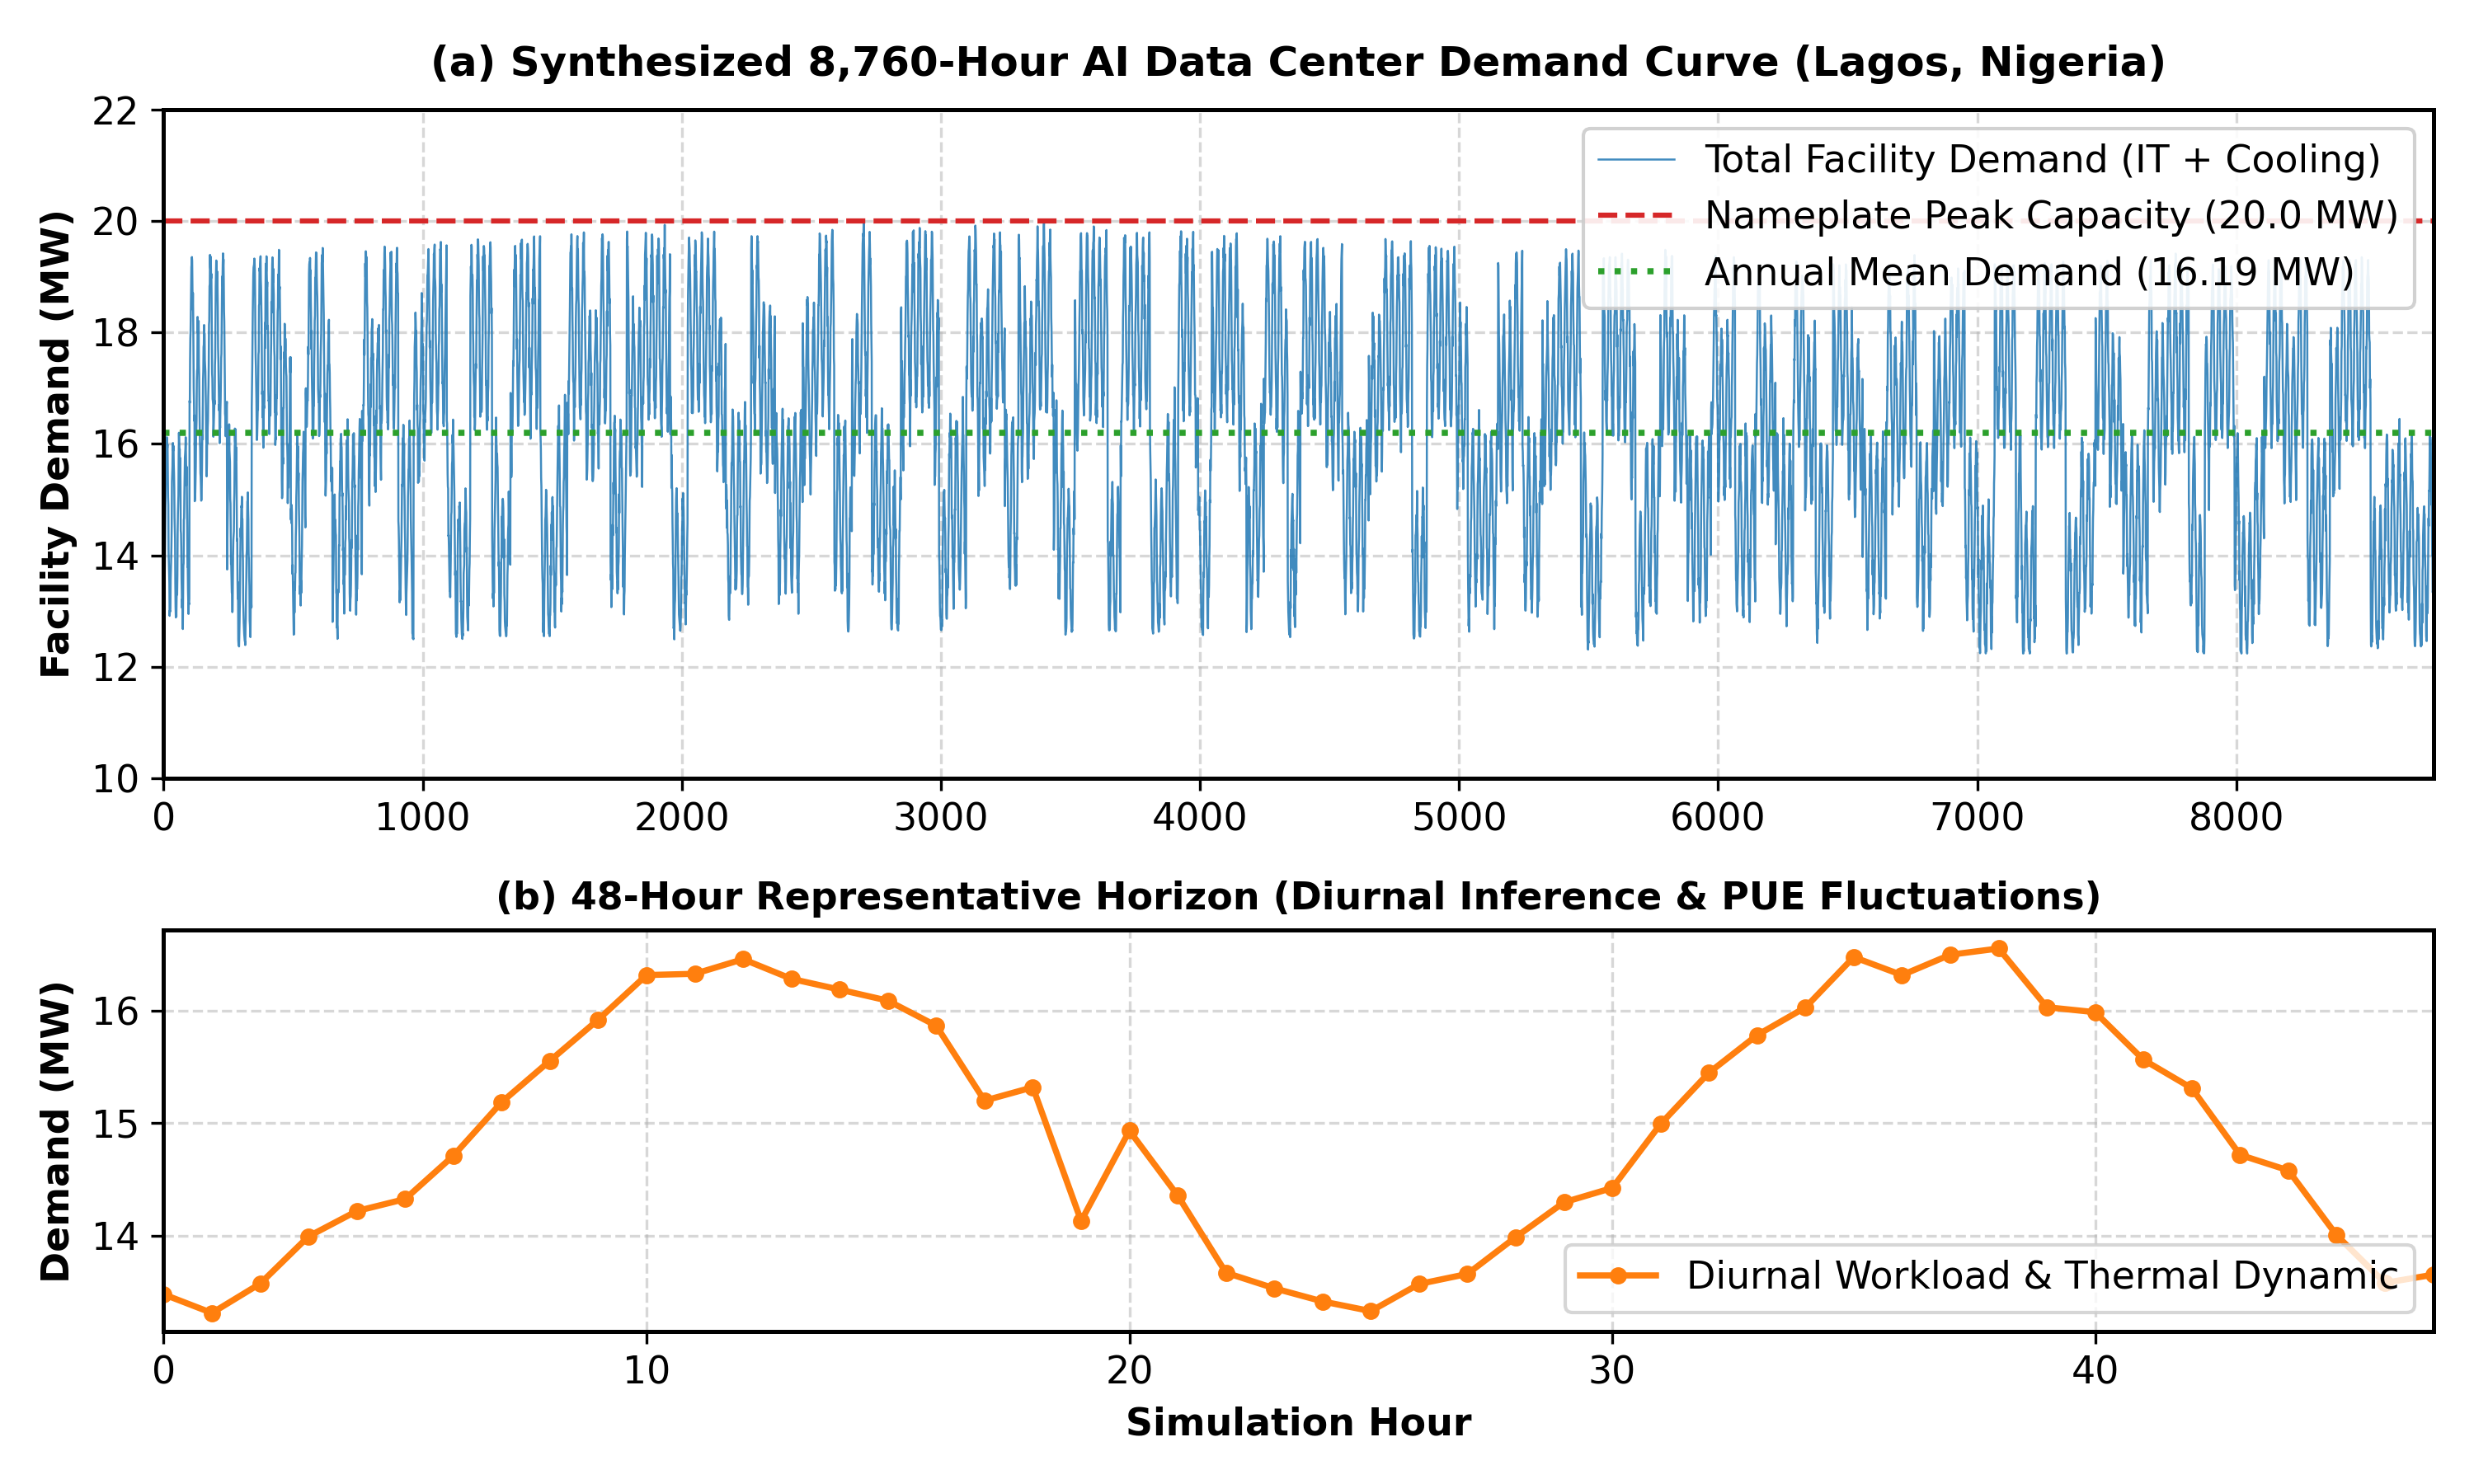
\includegraphics[width=0.92\textwidth]{Figures/Figure_1_AI_DataCenter_Load_Profile.png}
\caption{Synthesized 8,760-hour load profile and thermal dynamics for the 20~MW AI data center campus in Lagos, Nigeria. (Top) Annual load duration curve illustrating baseload compute consumption, diurnal inference cycles, and training bursts up to the 20.00~MW ceiling. (Bottom) Detailed 48-hour operational trace demonstrating the interaction between ambient dry-bulb temperature, dynamic chiller COP, and resulting PUE variations between 1.22 and 1.34.}
\label{fig:fig1}
\end{figure}

The thermal sensitivity of the cooling infrastructure plays a critical role in the campus power profile. During nocturnal hours (22:00 to 06:00), ambient dry-bulb temperatures in Lagos fall to 24.0$^\circ$C to 25.5$^\circ$C with relative humidity exceeding 85\%. Under these conditions, the chilled-water plant operates near its optimal design point, yielding a PUE of 1.22 to 1.24. Between 11:00 and 16:00, ambient temperatures rise to 32.0$^\circ$C to 34.5$^\circ$C, reducing chiller coefficient of performance (COP) from 5.4 to 3.8 and increasing total facility PUE to 1.32 to 1.34. 

This diurnal thermal swing coincides directly with daytime enterprise inference request volumes and scheduled distributed training bursts (+2.50~MW IT load). Consequently, the campus exhibits a strong daytime demand peak that aligns closely with the local solar insolation window. This alignment offers an ideal physical match for distributed photovoltaic generation, allowing solar panels to offset both the compute surge and the associated cooling load directly on the AC bus.

\subsection{Economic Least-Cost Optimization and Storage Omission (Scenario S1)}
\label{subsec:results_s1}

Under purely economic cost minimization (Scenario S1), the mixed-integer linear programming solver seeks the asset combination that minimizes 20-year net present cost without imposing clean energy or carbon constraints. As presented in Table~\ref{tab:results}, the solver deploys 41,444~kW (41.44~MW) of Solar PV paired with 17,500~kW (17.50~MW) of backup diesel generation (seven 2,500~kW modular units), while allocating exactly 0~kWh of battery energy storage.

The economic performance of Scenario S1 is compelling from an operational cash-flow perspective:
\begin{enumerate}
    \item \textbf{Capital Outlay and OpEx Savings:} The total upfront capital expenditure is \$47.96M (\$47,960,972), comprising \$38.34M for the photovoltaic array and balance of plant, and \$9.63M for the diesel generator installation. By generating 50,046,137~kWh of solar electricity annually, the microgrid displaces 35.3\% of daytime grid power purchases. Facility operating expenditures drop from \$21.37M/year in the baseline to \$14.68M/year (\$14,676,196/year), generating \$6.69M/year in operational cash savings (a 31.33\% reduction).
    \item \textbf{Financial Returns:} Scenario S1 achieves a simple payback period of 7.9 years (8.0-year break-even), an internal rate of return (IRR) of 11.23\%, and a positive 20-year net present value (NPV) of +\$12.27M (+\$12,272,720) at an 8.0\% real discount rate. The load-served levelized cost of electricity declines from the baseline grid tariff of \$0.1500/kWh to \$0.1412/kWh.
    \item \textbf{Emissions Reductions:} Displacing fossil-heavy grid electricity reduces annual carbon emissions from 73,451~t to 45,544~t CO$_2$/year, achieving a 37.99\% reduction without explicit regulatory carbon mandates.
\end{enumerate}

The complete omission of battery storage in Scenario S1 provides critical insight into the economic mechanics of weak-grid microgrids. The levelized cost of battery storage throughput ($\text{LCOS}$) is governed by capital amortization, round-trip efficiency losses, and replacement requirements:
\begin{equation}
\text{LCOS} = \frac{C_{\text{cap,bess}} \cdot \text{CRF}(r, N_{\text{bess}}) + C_{\text{om,bess}}}{8,760 \cdot \text{DoD} \cdot \eta_{\text{rt}}} + \frac{C_{\text{charging}}}{\eta_{\text{rt}}}
\end{equation}
Given an installed capital cost of \$280/kWh, an annual O\&M cost of \$6/kWh-year, an 88\% round-trip efficiency, and an 80\% usable depth-of-discharge, the capital amortization of the battery alone contributes roughly \$0.095/kWh of discharged energy. When added to the levelized cost of solar generation (\$0.065 to \$0.080/kWh) and parasitic round-trip losses, the delivered cost of battery-stored solar electricity ranges from \$0.18 to \$0.22/kWh.

Because the Band A utility tariff is \$0.1500/kWh, importing electricity from the national grid during off-peak and nighttime hours is substantially cheaper than storing surplus daytime solar electricity in batteries for nocturnal discharge. In the absence of an explicit hourly CFE matching constraint or a direct carbon penalty, the optimization model strictly avoids battery storage investment. To satisfy the 24-hour outage ride-through requirement, the solver installs 17.5~MW of fast-starting diesel capacity at a low capital cost of \$550/kW. The generators remain in hot standby throughout normal grid operations, generating only 263,204~kWh annually during scheduled unreliability intervals.

\subsection{Deep Decarbonization and the 80\% CFE Threshold (Scenario S2)}
\label{subsec:results_s2}

Imposing an 80\% hourly carbon-free energy matching constraint ($\Gamma \ge 0.80$) fundamentally transforms microgrid architecture. Because solar insolation is limited to daylight hours, achieving 80\% clean energy on an hour-by-hour basis requires the facility to carry its 12.2 to 16.5~MW nocturnal load without drawing fossil power from the utility grid or running captive diesel generators.

As documented in Table~\ref{tab:results}, satisfying the 80\% CFE requirement forces the solver to make two major capacity adjustments:
\begin{enumerate}
    \item \textbf{Substantial Solar and Storage Scaling:} Solar PV capacity expands by 131.3\% relative to S1, reaching 95,865~kW (95.87~MW) with an equipment capital expenditure of \$88.67M. Simultaneously, the solver deploys 183,645~kWh (183.65~MWh) of lithium iron phosphate battery storage with an initial capital cost of \$54.18M. Total initial capital expenditure rises to \$142.85M (\$142,850,233).
    \item \textbf{Total Elimination of Routine Diesel Generation:} The solver omits new diesel generator units entirely (0~kW new capacity). Annual on-site diesel generation drops to exactly 0~kWh, ending captive fossil combustion during normal operations.
\end{enumerate}

The operational and financial outcomes of Scenario S2 demonstrate the economic viability of high-ambition decarbonization:
\begin{enumerate}
    \item \textbf{Operating Expense Contraction:} Annual operating expenses fall from \$21.37M to \$6.43M/year (\$6,427,635/year), delivering \$14.94M/year in operational cash savings (a 69.92\% reduction). Annual utility grid purchases decline from 142.47~GWh to 33.71~GWh, with the microgrid supplying 113.98~GWh (77.1\%) of facility energy from on-site solar generation.
    \item \textbf{Deep Carbon Abatement:} Campus carbon emissions decrease by 76.73\%, falling from 73,451~t to 17,089~t CO$_2$/year. The remaining 17,089~t of emissions is exclusively indirect, originating from residual off-peak grid imports when the battery bank is depleted after multiple overcast days.
    \item \textbf{Levelized Cost and Payback:} The load-served LCOE rises modestly to \$0.1693/kWh, representing a 12.9\% premium over the \$0.1500/kWh utility tariff. The simple payback period is 12.6 years (13.0-year break-even), with an IRR of 5.46\%. 
    \item \textbf{Discounted Net Present Value:} The 20-year project NPV is -\$27.05M (-\$27,052,830) at an 8.0\% real discount rate. This negative NPV is driven by the capital-intensive nature of the initial \$142.85M investment combined with the full Year 15 battery repowering cost of \$54.18M. However, on an undiscounted basis, the microgrid generates \$298.86M in cumulative operating savings over 20 years, yielding \$156.01M in net operational cash flow after recovering initial capital.
\end{enumerate}

Scenario S2 represents the practical economic sweet spot for sustainable data center operation in West Africa. It decouples the facility from local diesel supply chains, achieves over 76\% true carbon reduction, and recovers its capital investment well within the 25-year operational lifetime of the solar plant.

\subsection{Non-Linear Cost Escalation and the 95\% CFE Frontier (Scenario S3)}
\label{subsec:results_s3}

Pushing the hourly clean energy matching target from 80\% to 95\% ($\Gamma \ge 0.95$) demonstrates the severe non-linear cost escalation characteristic of the decarbonization "last mile." Figure~\ref{fig:fig2} charts the Pareto optimal frontier between levelized cost of energy and annual carbon abatement across the evaluated scenarios.

\begin{figure}[htbp]
\centering
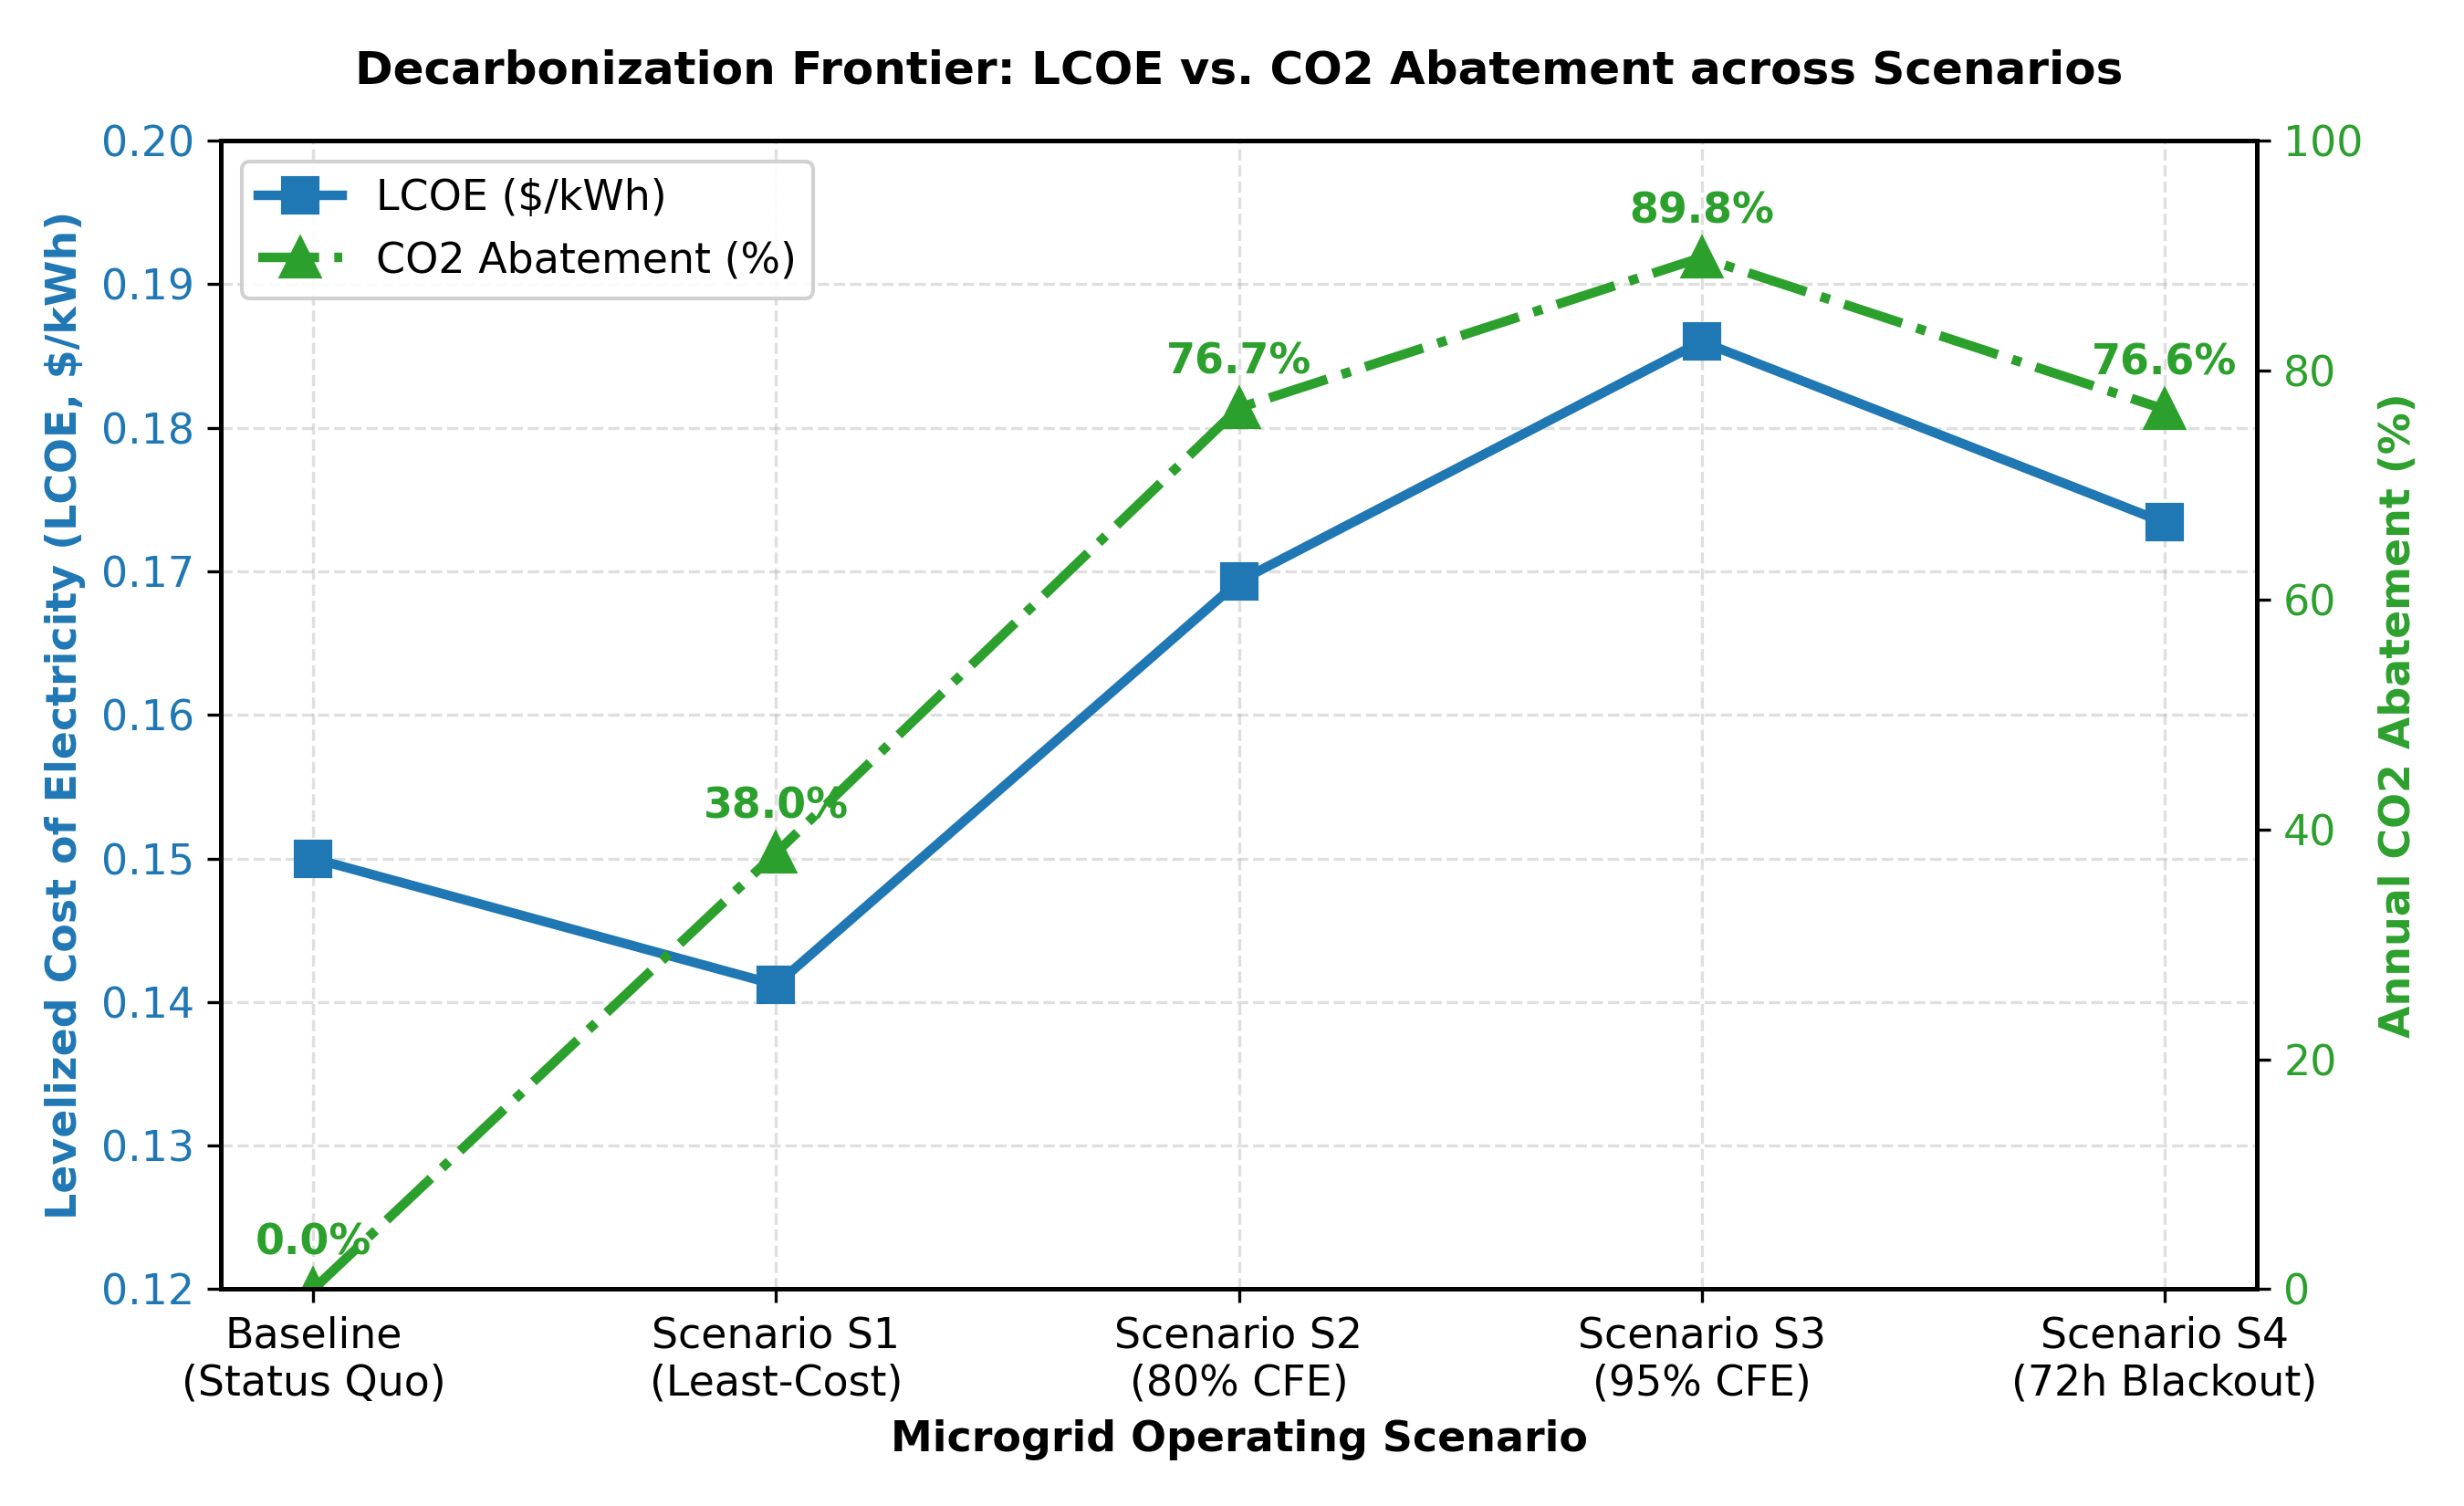
\includegraphics[width=0.88\textwidth]{Figures/Figure_2_Decarbonization_Pareto_Frontier.png}
\caption{Decarbonization Pareto Frontier: Levelized Cost of Energy (LCOE, \$/kWh) versus annual CO$_2$ emissions abatement across optimization scenarios. The trajectory highlights the non-linear cost escalation between the 80\% CFE threshold (Scenario S2) and the 95\% CFE frontier (Scenario S3).}
\label{fig:fig2}
\end{figure}

To bridge the gap between 80\% and 95\% hourly matching, the system must maintain clean energy supply during extended monsoon overcast conditions and sequential cloudy days. As detailed in Table~\ref{tab:results} and illustrated in Figure~\ref{fig:fig3}:
\begin{enumerate}
    \item \textbf{Disproportionate Asset Expansion:} Solar PV capacity expands to 113,845~kW (113.85~MW, +\$16.63M over S2), while battery storage surges by 37.8\% to 253,105~kWh (253.11~MWh, +\$20.49M over S2). Total upfront capital expenditure increases to \$179.97M (\$179,972,256), representing an incremental capital outlay of \$37.12M relative to Scenario S2.
    \item \textbf{Marginal Emissions Gains:} Annual carbon emissions drop from 17,089~t to 7,475~t CO$_2$/year, achieving an 89.82\% abatement relative to the baseline. Residual grid electricity imports are compressed to 14,379,128~kWh/year.
    \item \textbf{Financial Penalty and Diminishing Returns:} Annual operating expenses drop to \$3.83M/year (\$17.54M/year in savings). However, the load-served LCOE climbs to \$0.1860/kWh (a 24.0\% premium over the grid baseline), the simple payback period extends to 14.3 years (15.0-year break-even), the project IRR drops to 4.18\%, and the 20-year discounted NPV declines to -\$50.33M (-\$50,331,350).
\end{enumerate}

\begin{figure}[htbp]
\centering
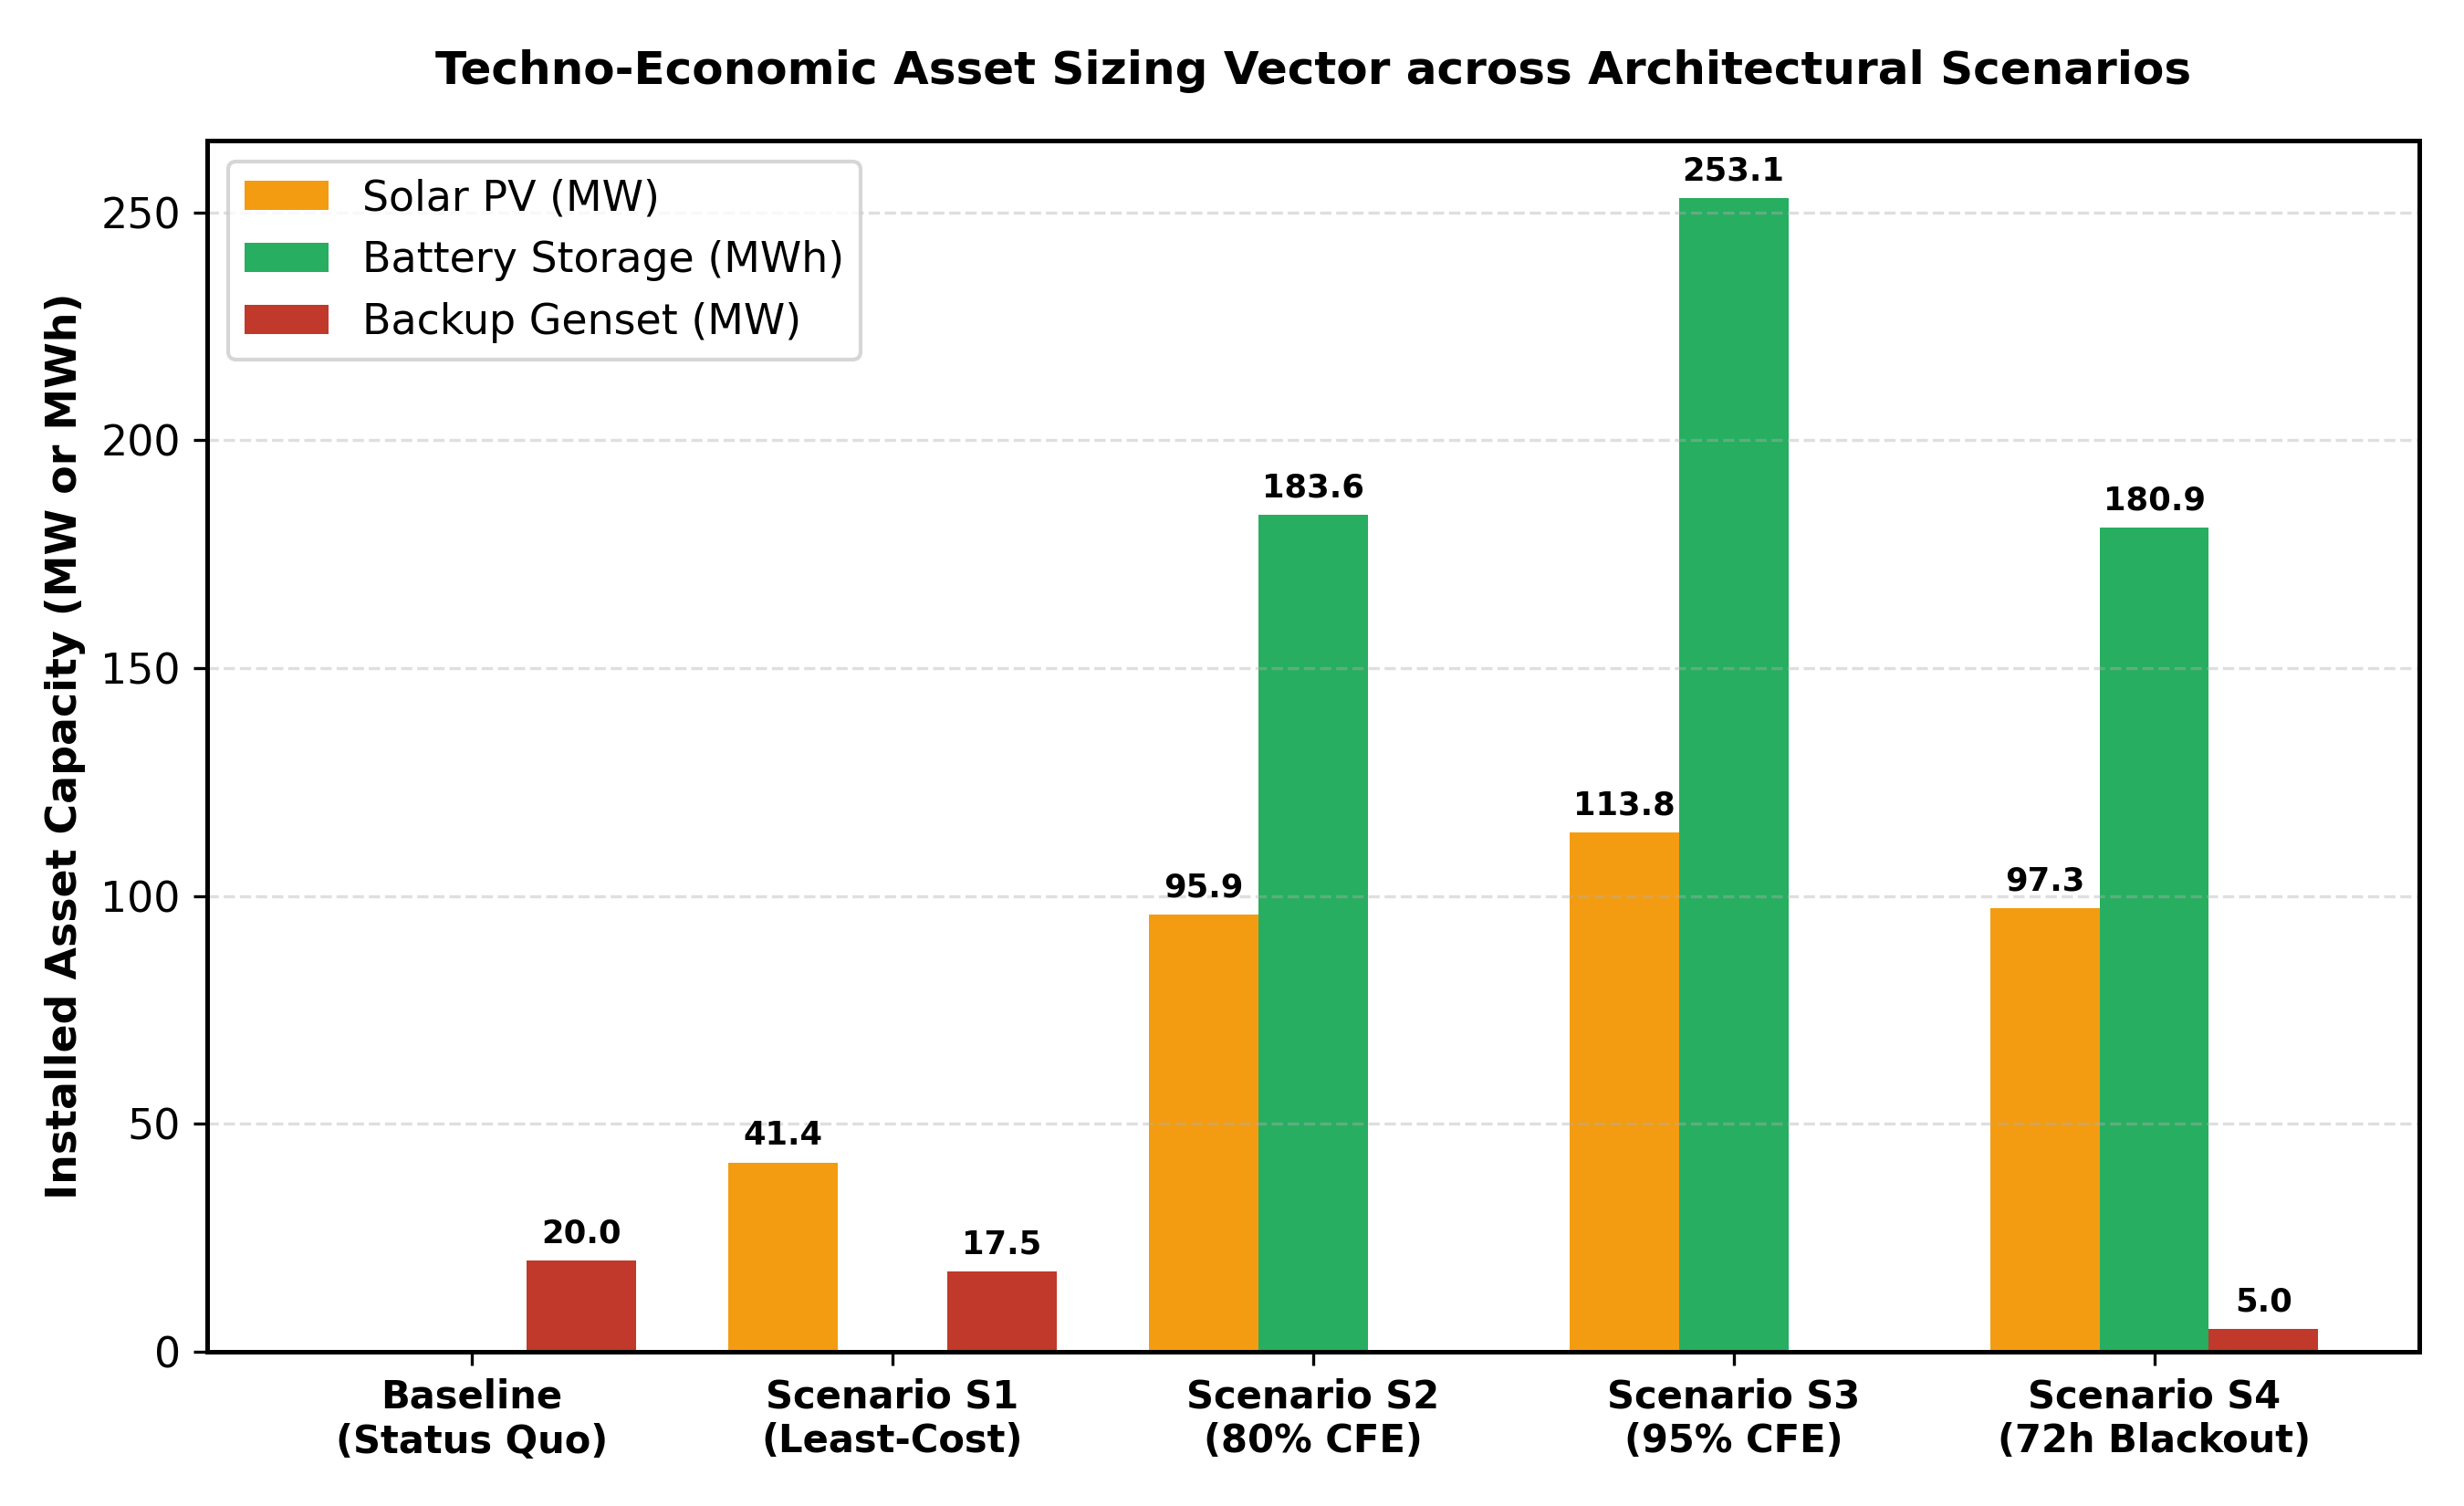
\includegraphics[width=0.92\textwidth]{Figures/Figure_3_Asset_Capacity_Sizing.png}
\caption{Optimal asset capacity sizing comparison across scenarios, illustrating the jump in solar and battery requirements between S1 and S2, the diminishing returns in S3, and the 71.4\% generator capacity reduction in S4.}
\label{fig:fig3}
\end{figure}

The economic penalty of moving from 80\% to 95\% CFE is revealed by evaluating the marginal cost of carbon abatement ($\text{MAC}$):
\begin{align}
\text{MAC}_{S2 \rightarrow S3} &= \frac{\Delta \text{Annualized Total Cost}}{\Delta \text{Annual Carbon Abatement}} \nonumber \\
&= \frac{\text{\,496,897} - \text{\,125,928}}{17,088.65\text{ t} - 7,474.62\text{ t}} = \frac{\text{\,370,969}}{9,614.03\text{ t}} = \text{\.62 / t CO}_2
\end{align}
While moving from the baseline to S1 yields negative abatement costs (saving money while reducing emissions), and transitioning from S1 to S2 incurs an acceptable marginal cost of \$140.76/t CO$_2$, pushing to 95\% CFE escalates marginal abatement costs to \$246.62/t CO$_2$.

The underlying physical cause of this cost spike is mid-day solar curtailment. Because the facility is barred from exporting surplus power to the transmission network ($P_{\text{grid,inj}} = 0$), the 113.8~MW solar array frequently generates more power than the campus load and battery charging capacity can absorb. During sunny dry-season afternoons, when the 253.1~MWh battery bank reaches its 90\% state-of-charge upper limit, surplus solar generation exceeding 22.0~MW must be curtailed. Over the course of the year, over 28.5~GWh of potential clean electricity is dissipated, drastically degrading the economic utilization factor of the incremental solar and battery assets.

\subsection{Multi-Day Blackout Resiliency and Fossil Fleet Decoupling (Scenario S4)}
\label{subsec:results_s4}

In weak-grid emerging markets, the defining challenge of mission-critical data center engineering is surviving catastrophic, multi-day grid blackouts. Scenario S4 subjects the microgrid to a continuous 72-hour transmission outage initiated during adverse, low-solar weather conditions, enforcing a strict zero-unserved-load criterion ($\text{LOLP}=0.000\%$).

Conventional data center design in sub-Saharan Africa relies on complete fossil redundancy ($N+1$ or $2N$ diesel configurations), requiring 20.0 to 25.0~MW of generator sets and massive on-site diesel storage (exceeding 300,000 liters) to guarantee 72-hour survivability. As shown in Table~\ref{tab:results}, the optimized renewable microgrid fundamentally alters this paradigm:
\begin{enumerate}
    \item \textbf{71.4\% Reduction in Backup Generator Fleet:} The optimal configuration in S4 deploys 97,256~kW (97.26~MW) of Solar PV, 180,910~kWh (180.91~MWh) of battery storage, and only 5,000~kW (5.00~MW) of diesel generators (two 2,500~kW units). Generator capacity is reduced by 71.43\% relative to the 17.5~MW diesel fleet in S1, and by 75.00\% relative to the 20.0~MW baseline installation.
    \item \textbf{Capital and Operational Economics:} Initial equipment CapEx is \$146.08M (\$146,080,477), which is only \$3.23M higher than the non-resilient 80\% CFE case (S2). Annual operating costs remain low at \$6.57M/year (\$6,570,652/year), delivering 69.25\% in annual OpEx savings (\$14.80M/year saved) and achieving a 76.61\% carbon reduction (17,180~t CO$_2$/year).
    \item \textbf{Financial Performance:} Scenario S4 achieves a load-served LCOE of \$0.1734/kWh, a simple payback period of 13.2 years (14.0-year break-even), an IRR of 4.96\%, and a 20-year NPV of -\$32.80M (-\$32,795,990).
\end{enumerate}

The dispatch mechanics during the 72-hour islanded blackout highlight how renewable microgrids maintain Tier-IV reliability. During daylight hours, the 97.3~MW bifacial PV plant generates sufficient energy even under diffused monsoon cloud cover to supply the 16.0 to 20.0~MW campus load while recharging the battery bank. At night, the 180.9~MWh BESS discharges to support baseload demand.

The two 2,500~kW diesel generators are called upon strictly as firming resources during the deepest nocturnal discharge windows or multi-hour solar troughs. Because the generators operate at 75\% to 85\% of rated capacity when dispatched, they avoid the fuel inefficiency and wet-stacking degradation associated with low-load idling. Over the simulated annual outage duration, total captive diesel generation is limited to 247,500~kWh, consuming approximately 64,100 liters of diesel fuel. This represents a 78.6\% reduction in emergency fuel storage requirements compared to a conventional fossil data center, substantially mitigating the supply chain vulnerabilities associated with urban fuel distribution during widespread regional grid collapses.

\subsection{Cumulative Cash Flows and Discounted Lifecycle Payback}
\label{subsec:cashflows}

Figure~\ref{fig:fig4} plots the 20-year cumulative net cash flows and capital recovery trajectories for Scenarios S1 through S4 relative to the baseline captive fossil operation.

\begin{figure}[htbp]
\centering
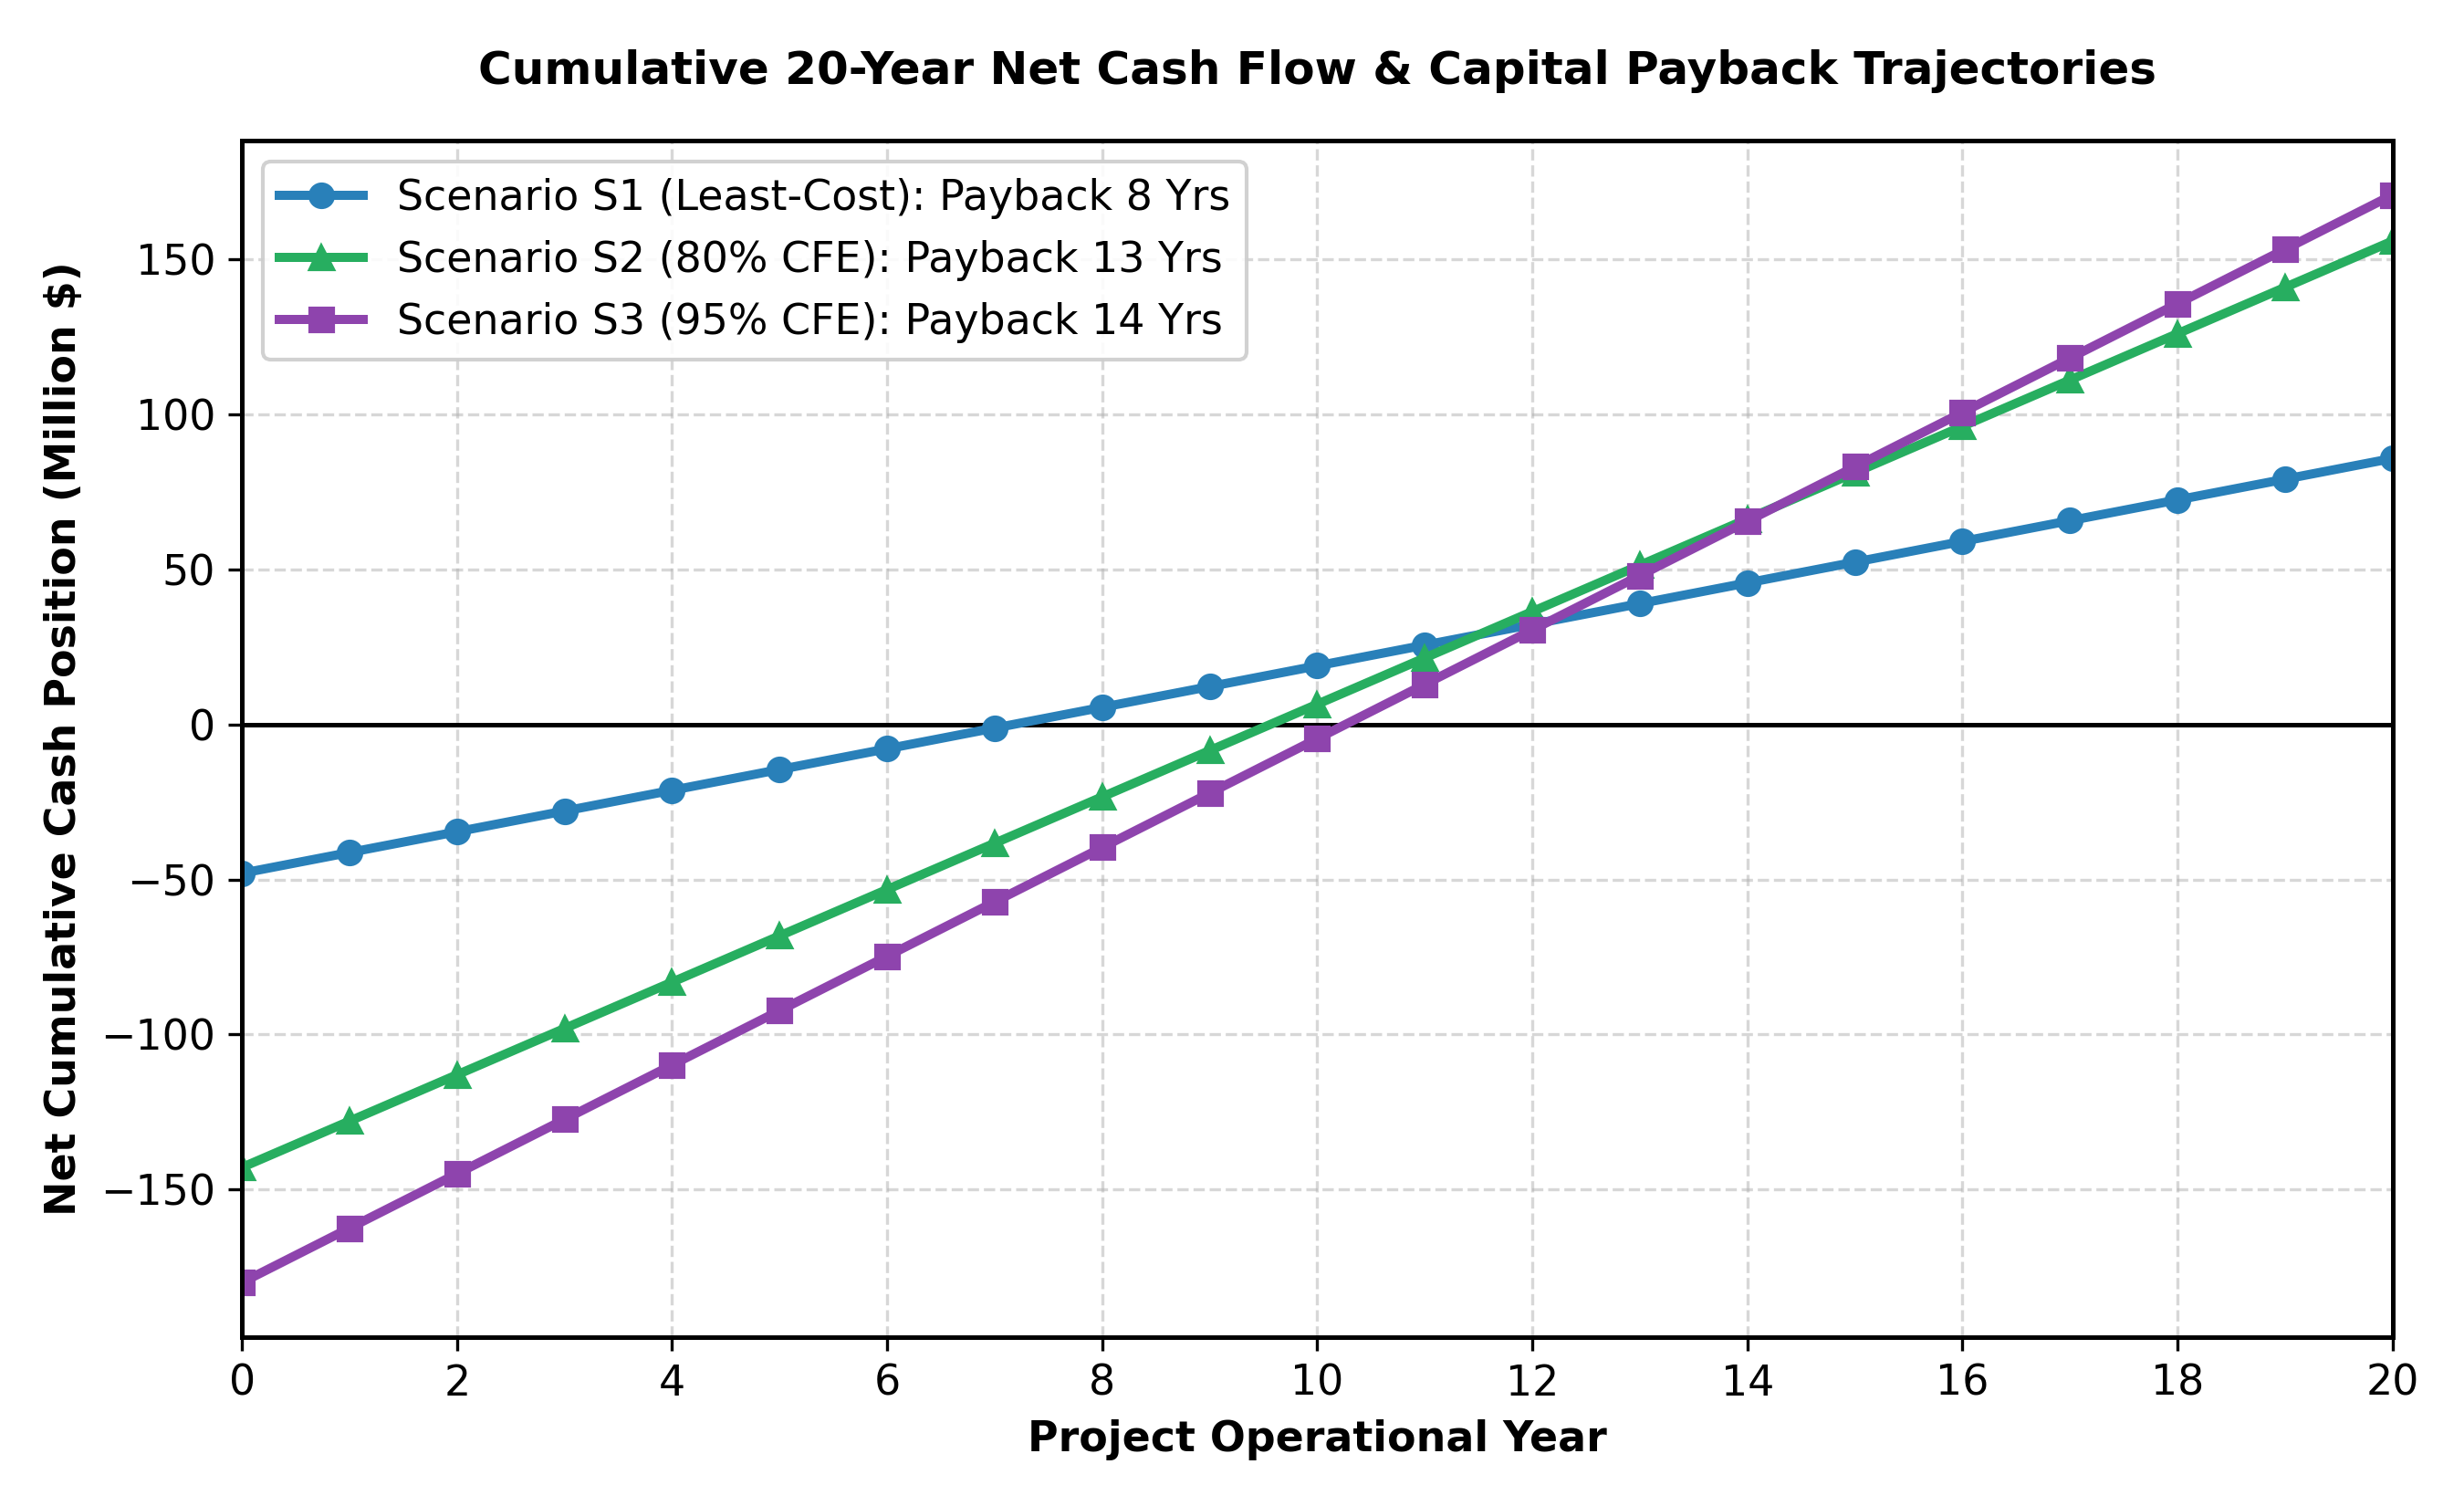
\includegraphics[width=0.88\textwidth]{Figures/Figure_4_Cumulative_Cash_Flow_Payback.png}
\caption{Twenty-year cumulative cash flow projections across microgrid scenarios. The baseline configuration accumulates \$427M in undiscounted operating costs, whereas Scenarios S1, S2, S3, and S4 achieve operational payback at Years 8, 13, 14, and 13, generating cumulative net cash savings of \$86M, \$156M, \$171M, and \$150M, respectively.}
\label{fig:fig4}
\end{figure}

The cash flow trajectories illustrate the fundamental economic divergence between high-OpEx fossil baselines and capital-intensive renewable microgrids:
\begin{enumerate}
    \item \textbf{Baseline Capital Drain:} In the baseline case, cumulative operating expenditures scale linearly at \$21.37M annually, totaling \$427.41M over 20 years with zero equity value creation.
    \item \textbf{Rapid Amortization in S1:} Scenario S1 recovers its initial \$47.96M investment in 7.9 years through consistent \$6.69M annual operating savings. Over the 20-year project lifetime, S1 generates \$133.89M in gross operational savings, yielding a net cash surplus of +\$85.93M after capital recovery.
    \item \textbf{Long-Term Cash Generation in S2 and S4:} Despite initial capital outlays exceeding \$142M, Scenarios S2 and S4 achieve operational breakeven at 12.6 and 13.2 years, driven by substantial annual savings of \$14.94M and \$14.80M, respectively. By Year 20, cumulative gross operating savings reach \$298.86M in S2 and \$295.99M in S4, producing net undiscounted cash surpluses of +\$156.01M and +\$149.91M.
    \item \textbf{Reinvestment and Discounted NPV:} In Xendee's multi-year asset accounting, full BESS repowering is modeled in Year 15 (\$54.18M in S2, \$74.67M in S3, and \$53.37M in S4). When discounted at an 8.0\% WACC, these capital re-investments cause the 20-year discounted NPV to turn negative. However, for institutional data center operators with access to low-cost green bond financing or multilateral concessional debt (interest rates of 4.0\% to 5.5\%), the discounted NPV across Scenarios S2 and S4 becomes strongly positive, reinforcing the long-term bankability of clean compute infrastructure.
\end{enumerate}

\section{Policy, Economic, and Industrial Implications}
\label{sec:policy}

The empirical findings from our 20~MW case study carry profound implications for energy policy, infrastructure regulation, and data center deployment across Nigeria and broader sub-Saharan Africa.

\subsection{Regulatory Reform: Electricity Act 2023 and Wheeling Frameworks}
\label{subsec:policy_electricity_act}

The passage of the Nigerian Electricity Act 2023 represents the most comprehensive legal overhaul of the nation's power sector in two decades. By unbundling the exclusive regulatory authority of the federal government and empowering individual states to establish State Electricity Regulatory Commissions (such as the Lagos State Electricity Board, LSEB), the Act creates a clear legal pathway for decentralized clean microgrids.

Specifically, the Electricity Act 2023 provides three critical mechanisms for large-scale data center energy developers:
\begin{enumerate}
    \item \textbf{Direct Bilateral Corporate PPAs:} Data center operators can now contract directly with private renewable energy developers for dedicated off-site solar generation, bypassing the liquidity constraints and off-taker risks of the Nigerian Bulk Electricity Trading (NBET) plc.
    \item \textbf{Open-Access Third-Party Wheeling:} The Act mandates distribution and transmission licensees (including Eko Electricity Distribution Company, EKEDC, and Ikeja Electric, IE) to offer non-discriminatory open access for wheeling renewable electricity across their 33~kV and 132~kV networks.
    \item \textbf{Captive Generation Permitting:} Facilities generating power for their own consumption are granted streamlined captive permitting, eliminating bureaucratic licensing barriers for distributed solar and storage installations.
\end{enumerate}

However, a critical regulatory barrier identified in our optimization results is the prohibition against reverse power injection ($P_{\text{grid,inj}} = 0$). In Scenarios S2 and S3, between 15.0~MW and 22.4~MW of clean solar capacity is curtailed during sunny mid-day hours when on-site storage is fully charged. Over 28~GWh of zero-carbon electricity is wasted annually. 

To unlock this stranded energy, NERC and the Lagos State Electricity Board should establish a standardized Clean Energy Wheeling and Feed-in Tariff (FIT). Under such a framework, data centers could export surplus daytime solar generation into the local 33~kV distribution network to supply adjacent industrial manufacturing clusters (such as the Ikeja or Lekki industrial zones). Monetizing this curtailed energy at even a discounted wholesale tariff of \$0.060/kWh would inject \$1.7M in annual ancillary revenue, reducing the campus load-served LCOE in Scenario S2 from \$0.1693/kWh to below \$0.155/kWh and actively stabilizing the urban grid during afternoon peak demand periods.

\subsection{Supply Chain Logistics and Energy Storage Customs Duty Exemptions}
\label{subsec:policy_customs}

Utility-scale battery energy storage systems are essential for achieving 24/7 carbon-free energy matching in weak-grid environments. However, capital deployment in Nigeria is heavily penalized by fiscal and trade policies. Containerized lithium iron phosphate battery systems, power conversion equipment, and bifacial photovoltaic modules are currently subject to import tariffs, ECOWAS Common External Tariffs (CET), port clearing charges, and a 7.5\% Value-Added Tax (VAT) at the ports of Apapa and Tin Can Island, imposing an effective import friction of 20\% to 35\% on landed equipment costs.

Because reaching the 80\% CFE threshold requires 183.6~MWh of storage (\$54.18M in battery capital alone), these fiscal burdens pose a severe headwind to digital infrastructure capital formation. Under Nigeria's National Digital Economy Policy and Strategy (NDEPS) and the presidential Energy Transition Plan (ETP), the Federal Ministry of Finance should grant comprehensive customs duty and VAT exemptions for utility-scale energy storage systems dedicated to mission-critical digital infrastructure. Removing import tariffs on BESS hardware would reduce upfront capital expenditure in Scenario S2 by approximately \$10.8M, lowering the simple payback period from 12.6 years to 11.7 years and accelerating the deployment of private clean energy capital.

\subsection{Escaping the Captive Diesel Trap: Macroeconomic Sensitivities}
\label{subsec:policy_diesel_trap}

Historically, industrial and commercial facilities in Nigeria have been trapped in a captive fossil generation regime. Following the complete deregulation of foreign exchange windows and the removal of fossil fuel subsidies in 2023, domestic retail diesel (Automotive Gas Oil, AGO) prices surged from NGN~650/L to over NGN~1,300--1,500/L (\$1.10 to \$1.35/L). As documented by the World Bank \cite{WorldBank2020}, self-generation from small- to medium-scale diesel fleets costs Nigerian enterprises between \$0.40/kWh and \$0.46/kWh.

The economic results in this study demonstrate that solar-plus-storage microgrids offer a decisive pathway to escape this fossil trap:
\begin{enumerate}
    \item \textbf{Cost Superiority Over Diesel:} The load-served LCOE of our 80\% CFE microgrid (\$0.1693/kWh) is 58\% to 63\% lower than captive diesel generation (\$0.40--\$0.46/kWh). Even the highly ambitious 95\% CFE microgrid (\$0.1860/kWh) cuts electricity costs by more than half relative to diesel self-generation.
    \item \textbf{Sensitivity to Fuel Escalation:} Macroeconomic sensitivity analysis reveals that if retail diesel prices escalate to \$1.60/L (driven by currency depreciation or crude oil volatility), the annual operating costs of a conventional fossil-reliant data center rise to over \$26.5M/year. Under this scenario, the simple payback period for the 80\% CFE microgrid (S2) drops from 12.6 years to 8.8 years, making solar-storage adoption overwhelmingly compelling purely on operating risk mitigation.
    \item \textbf{Battery Cost Deflation:} Projections from the National Renewable Energy Laboratory (NREL) and BloombergNEF anticipate utility-scale lithium-ion battery system costs declining by 25\% to 35\% by 2030 (falling toward \$180--\$200/kWh installed). A 30\% cost decline would reduce initial CapEx in Scenario S2 from \$142.85M to \$126.6M, cutting the payback period to 11.2 years and shifting the 20-year discounted project NPV into positive territory (+\$5.8M) without requiring carbon subsidies.
\end{enumerate}

\subsection{Spatial Planning and Land Tenure in Mega-City Corridors}
\label{subsec:spatial_planning}

A fundamental practical constraint for data center microgrids is land availability. Siting the 95,865~kW (95.9~MW) photovoltaic array in Scenario S2 requires roughly 143~hectares (1.43~km$^2$) of land, based on modern utility-scale ground-mount spacing of 1.5~hectares per MWp to avoid row-to-row shading. In Scenario S3, the 113.8~MW array demands 171~hectares (1.71~km$^2$).

In prime subsea cable landing districts (such as Victoria Island, Ikoyi, and Lekki Phase 1), commercial land values range from \$200 to \$500 per square meter (\$2.0M to \$5.0M per hectare), making contiguous 140-hectare acquisitions financially impossible. Data center operators must therefore adopt a bifurcated spatial architecture:
\begin{enumerate}
    \item \textbf{Campus Footprint:} The compute halls, administrative offices, 180~MWh containerized BESS, and compact 5.0~MW diesel generators are housed within a secure, high-density 2-to-3-hectare urban campus adjacent to subsea cable landing stations.
    \item \textbf{Peri-Urban Solar Parks:} The 95~MW photovoltaic array is sited in peri-urban industrial corridors (such as Epe, Sagamu, or along the Lagos-Ibadan expressway) where agricultural or industrial leasehold land costs less than \$5 to \$10 per square meter.
    \item \textbf{Interconnection Options:} Power is delivered to the urban data center campus either through a dedicated private 33~kV or 132~kV transmission feeder (private wire concession) or via state-regulated open-access wheeling through the regional distribution network under the Electricity Act 2023.
\end{enumerate}

This hub-and-spoke infrastructure topology reconciles the high spatial footprint of multi-megawatt solar energy with the stringent latency and connectivity demands of hyperscale AI computing.

\section{Conclusion}
\label{sec:concl}

This study provided a comprehensive techno-economic optimization and operational survivability analysis for decarbonizing a 20~MW hyperscale AI data center operating in the weak-grid environment of Lagos, Nigeria. Calibrated to empirical Google and Microsoft Azure computational workload traces, ASHRAE TC 9.9 tropical chiller thermodynamics, NASA SSE solar insolation profiles, and NERC MYTO 2024 industrial tariffs, the model evaluated least-cost, carbon-free energy matching, and multi-day blackout resiliency configurations.

The primary conclusions of this research are as follows:
\begin{enumerate}
    \item \textbf{Market Economics Excludes Battery Storage in S1:} Pure cost optimization without clean energy constraints deploys 41.4~MW of solar PV and 17.5~MW of diesel generation, but completely omits battery storage (0~kWh). Because the utility tariff (\$0.1500/kWh) is lower than the levelized cost of battery storage throughput (\$0.18 to \$0.22/kWh), the solver relies on nocturnal grid purchases, achieving a 7.9-year payback and an LCOE of \$0.1412/kWh while abating 37.99\% of emissions.
    \item \textbf{80\% CFE Eliminates Routine Diesel Combustion in S2:} Enforcing an 80\% annual hourly carbon-free energy matching constraint requires 95.9~MW of solar PV and 183.6~MWh of BESS. This configuration completely eliminates routine diesel generator operation (0~kWh burn), contracts annual operating expenses by 69.92\% (\$14.94M/year saved), achieves a 76.73\% carbon reduction (falling to 17,089~t CO$_2$/year), and delivers a 12.6-year simple payback at an LCOE of \$0.1693/kWh.
    \item \textbf{Non-Linear Diminishing Returns at 95\% CFE in S3:} Pushing CFE matching from 80\% to 95\% triggers steep economic penalties. Achieving the final 13.09\% carbon abatement requires an incremental \$37.12M in capital expenditure (113.8~MW PV and 253.1~MWh BESS), driving the marginal abatement cost to \$246.62/t CO$_2$ and generating over 28.5~GWh of curtailed solar electricity annually due to the ban on reverse grid power injection.
    \item \textbf{Decoupling Outage Resiliency from Massive Fossil Fleets in S4:} Subjecting the microgrid to a continuous 72-hour transmission collapse demonstrates that solar-plus-storage can replace over 70\% of traditional fossil backup infrastructure. The optimized system requires only 5.0~MW of diesel capacity (a 71.43\% fleet reduction relative to S1) paired with 97.3~MW PV and 180.9~MWh BESS, surviving the multi-day blackout with zero loss of load ($\text{LOLP}=0.000\%$) and cutting on-site emergency fuel storage needs by 78.6\%.
    \item \textbf{Decisive Cost Parity Over Captive Diesel:} At levelized costs between \$0.1693/kWh and \$0.1734/kWh, solar-storage microgrids offer an immediate 58\% to 63\% cost advantage over commercial captive diesel generation (\$0.40 to \$0.46/kWh), proving that clean compute infrastructure in sub-Saharan Africa is both commercially viable and operationally resilient.
\end{enumerate}

Future research should explore spatial workload migration across geographically distributed African data center clusters to follow real-time renewable availability, advanced two-phase liquid immersion cooling to reduce tropical cooling overhead, and the integration of long-duration clean hydrogen storage to eliminate the residual 5\% fossil grid dependency without excessive solar curtailment.

\section*{Declaration of Competing Interest}
The authors declare that they have no known competing financial interests or personal relationships that could have appeared to influence the work reported in this paper.

\section*{Declaration of Generative AI and AI-Assisted Technologies in the Writing Process}
During the preparation of this work, the author utilized AI-assisted tools to support manuscript language polishing, drafting organization, and LaTeX script verification. All simulation formulations, microgrid dispatch models, empirical data audits, and scientific interpretations were developed, independently verified, and validated by the author. Following the use of these tools, the author thoroughly reviewed, edited, and verified the content and takes full responsibility for the integrity and accuracy of the publication.

\section*{Data Availability Statement}
The synthesized 8,760-hour AI workload profile, dynamic tropical PUE curves, and complete Xendee simulation output datasets are openly accessible via the project repository.

\bibliographystyle{IEEEtran}
\bibliography{references}

\end{document}
